% !TeX spellcheck = en_GB
%%%%%%%%%%%%%%%%%%%%%%%%%%%%%%%%%%%%%%%%%%%%%%%%%%%%%%%%%%%%%%%%%%%%%%%%%%
%%%%%%%%% Synoptic Phenomena observed? %%%%%%%%%%%%%%
\section{Observation and predictions of large scale weather phenomena at the surface}\label{sec:res:large_scale_sfc}
\textcolor{red}{What is the goal of this section?}
One of the main factors, that made the Christmas 2016 storm so interesting is the fact that fronts passed over Norway during the six-day period. One aim of this thesis is to identify if large scale phenomena were observed at the measurement site and if MEPS predicted the same measured pressure, temperature, wind, and precipitation patterns during the extreme event. 
\\
A comparison between the surface observations at Haukeliseter and the ECMWF analysis of the dynamic tropopause and geopotential thickness maps show that frontal transitions occurred on three days during the 2016 Christmas storm, \num{23}, \num{25}, and \SI{26}{\dec} (\Cref{sec:largeScale}).  
These show in the measurements and MEPS ensemble forecasts on \num{23}, \num{25}, and \SI{26}{\dec} (\Cref{fig:res:sfc_obs_meps}). 
\\
\Cref{fig:res:sfc_obs_meps} shows the different parameters forecasts initialised at \SI{00}{\UTC} for \num{23}, \num{25}, and \SI{26}{\dec}, as well as the observations at the Haukeliseter measurement site.
Pressure decreases and increases, as well as temperature increases, and wind changes are present on \num{23} and \SI{26}{\dec}, since these changes show in the surface observations in \Cref{fig:res:sfc_obs_meps}, it is assumed that frontal boundaries passed. The \SI{25}{\dec} shows an increase of temperature between \SIlist{15;17}{\UTC} leading to the assumption of a warm air evolution in \Cref{fig:res:sfc_temp25}. The overall weather situation, described in \Cref{sec:largeScale}, showed that a warm front as well as cold front influenced Norway, on \SI{25}{\dec}. But since the pressure and wind does not indicate a change related to frontal conversion, it is assumed that only the warm air section between the frontal boundaries showed in the surface measurements at Haukeliseter.   
\\
As described in \Cref{sec:largeScale} the ECMWF dynamic tropopause analysis (\Cref{fig:DT23}) shows more ridging at the DT level on \SI{23}{\dec}, than on the previous days. Warm air is advected closer over to Southern Norway \Cref{fig:DT23}. The low-pressure system approaches in the course of the day south-east of Iceland and hence stronger west to south west wind are associated with the cyclone (\Cref{fig:GP23}). The MEPS forecast, initialised on \SI{23}{\dec} at \SI{0}{\UTC} in \Cref{fig:res:sfc_pres23} follows the observations and shows the decrease in pressure after \SI{12}{\UTC} due to the transition of the occluded front with a constant pressure after the transition. Since warmer air is more advected to the north and the DT in \Cref{fig:DT23} shows a warm low-pressure core, an increase in temperature is observed and predicted at the measurement site (\Cref{fig:res:sfc_temp23}). \textcolor{red}{Include L, H in the surface pressure images}
%%%%%%% image sfc obs  %%%%%%%%%%%%%%%%
\begin{figure}[H]
	\centering
	% sfc pressure
	\begin{subfigure}[b]{0.49\textwidth}
		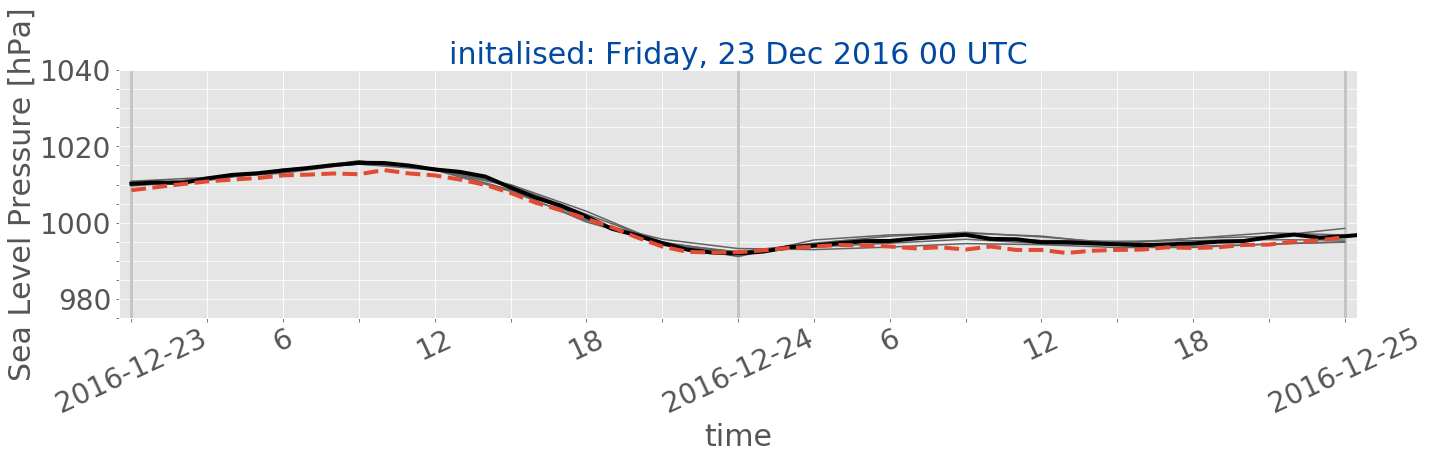
\includegraphics[trim={0.cm 5.cm 0cm 0cm},clip,
		width=\textwidth]{./fig_sfc_pressure/20161223_00}
		\caption{}\label{fig:res:sfc_pres23}
	\end{subfigure}
	%
	\begin{subfigure}[b]{0.49\textwidth}
		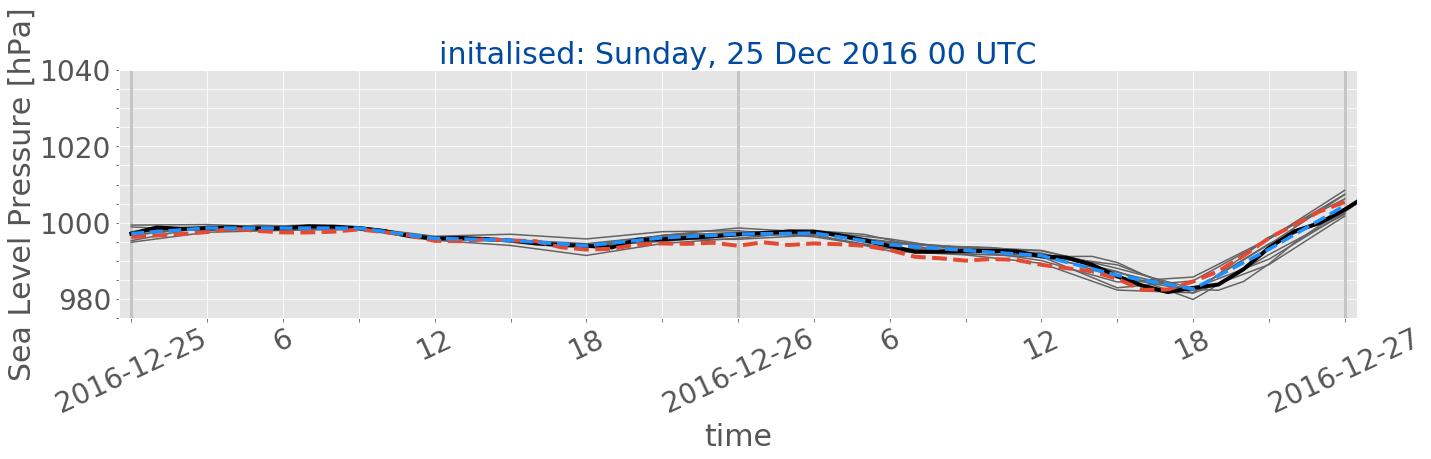
\includegraphics[trim={0.cm 5.cm 0cm 0cm},clip,
		width=\textwidth]{./fig_sfc_pressure/20161225_00}
		\caption{}\label{fig:res:sfc_pres25}
	\end{subfigure}
	% sfc temp
	\begin{subfigure}[b]{0.49\textwidth}
		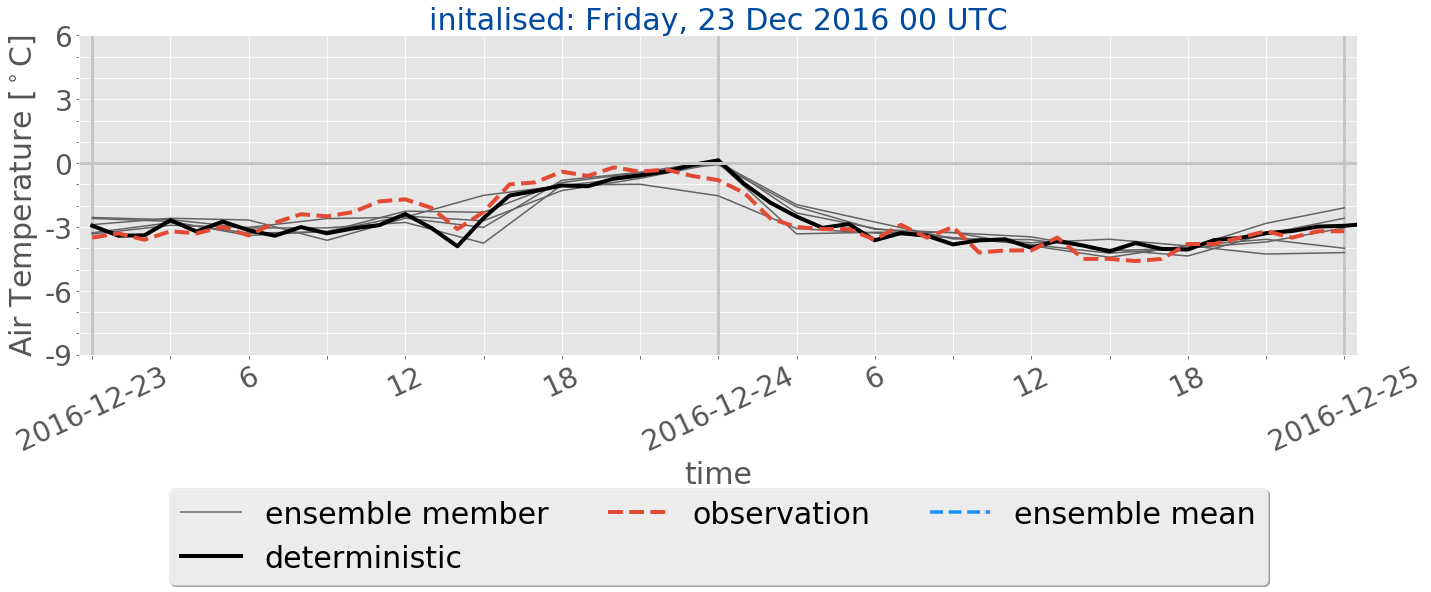
\includegraphics[trim={0.cm 5.cm 0cm 0cm},clip,
		width=\textwidth]{./fig_sfc_temp/20161223_00}
		\caption{}\label{fig:res:sfc_temp23}
	\end{subfigure}
	%
	\begin{subfigure}[b]{0.49\textwidth}
		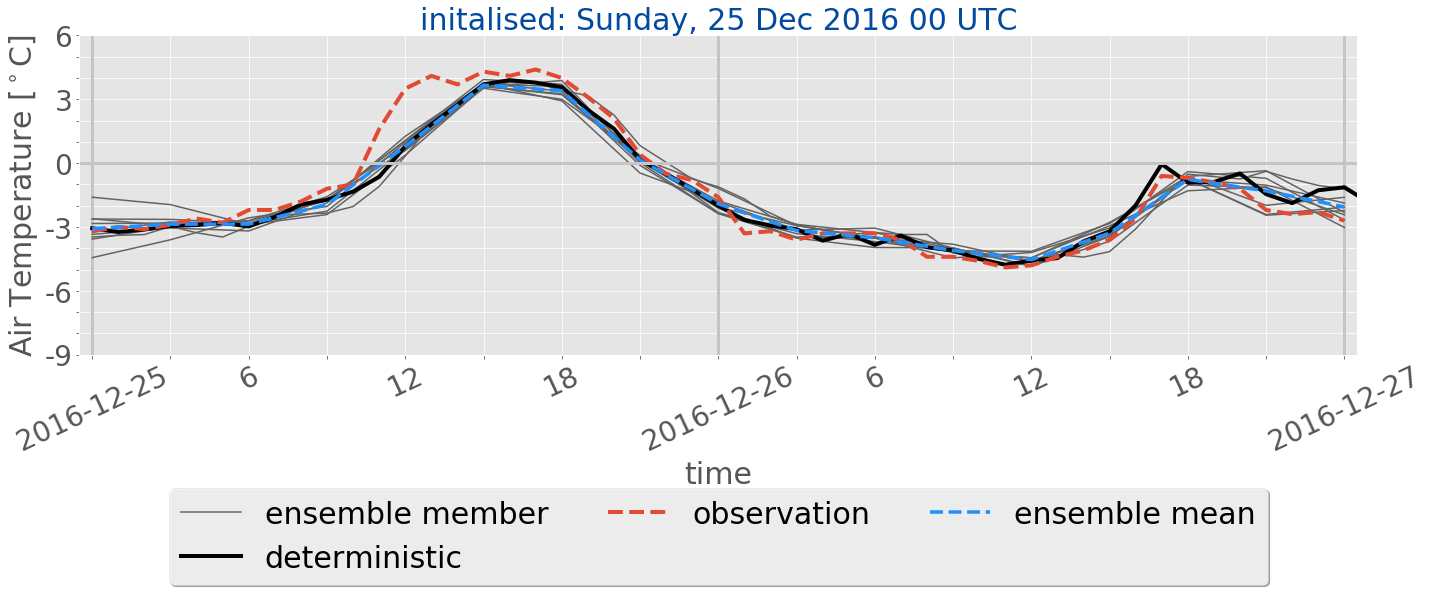
\includegraphics[trim={0.cm 5.cm 0cm 0cm},clip,
		width=\textwidth]{./fig_sfc_temp/20161225_00}
		\caption{}\label{fig:res:sfc_temp25}
	\end{subfigure}
	% sfc wd
	\begin{subfigure}[b]{0.49\textwidth}
		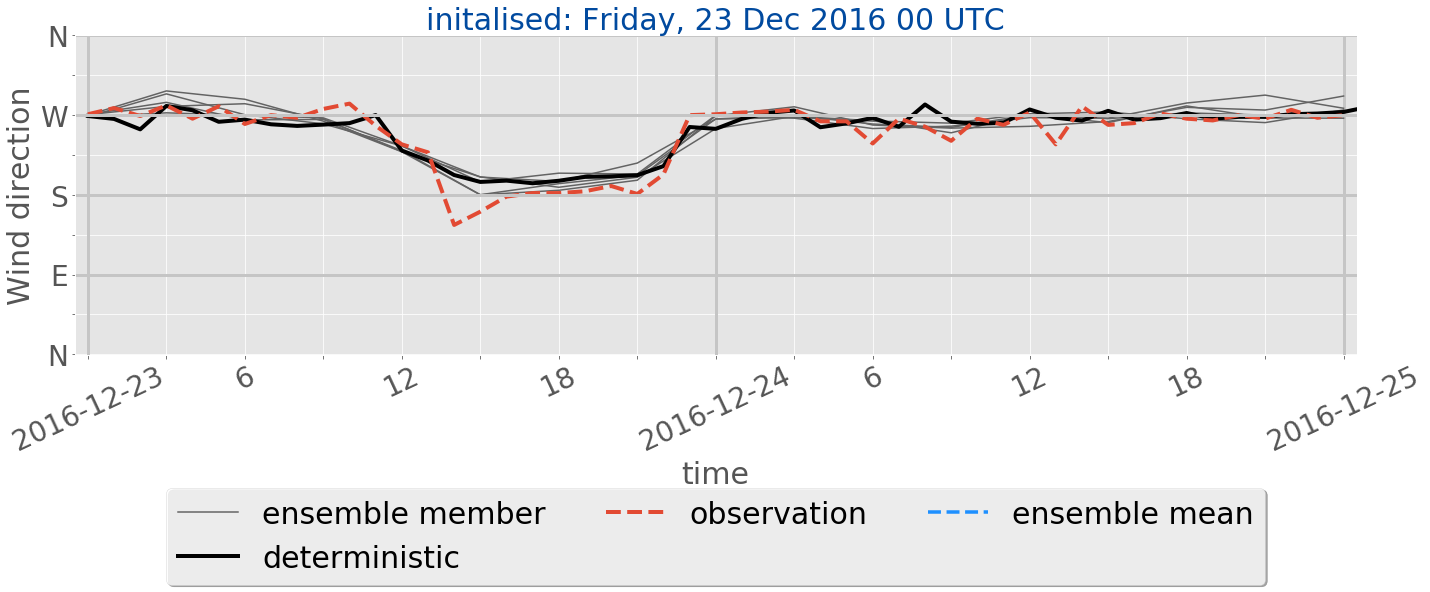
\includegraphics[trim={0.cm 5.cm 0cm 0cm},clip,
		width=\textwidth]{./fig_sfc_wd/20161223_00}
		\caption{}\label{fig:res:sfc_wd23}
	\end{subfigure}
	%
	\begin{subfigure}[b]{0.49\textwidth}
		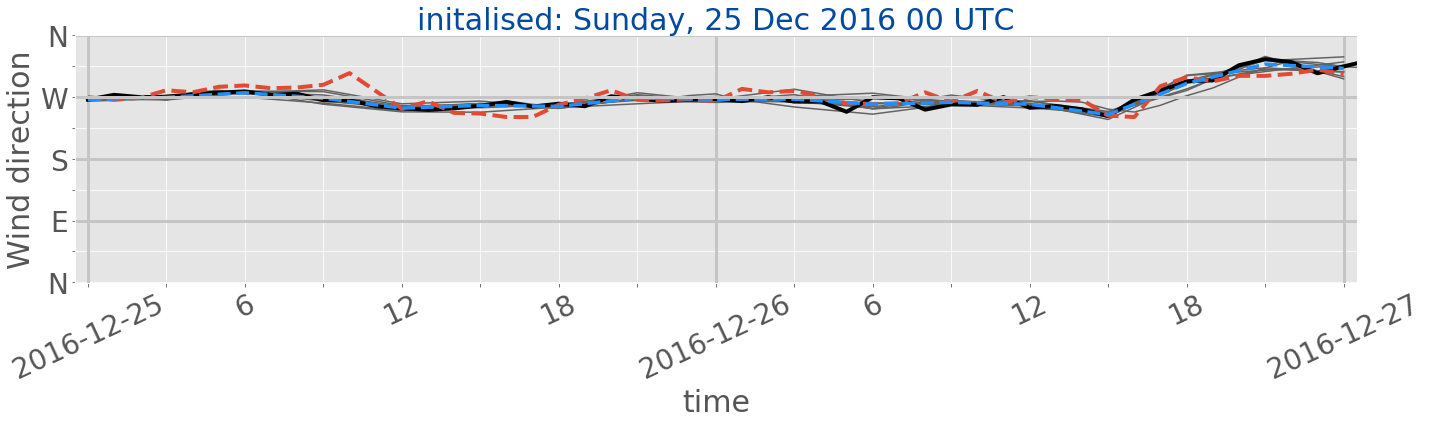
\includegraphics[trim={0.cm 5.cm 0cm 0cm},clip,
		width=\textwidth]{./fig_sfc_wd/20161225_00}
		\caption{}\label{fig:res:sfc_wd25}
	\end{subfigure}
	% sfc ws
	\begin{subfigure}[b]{0.49\textwidth}
		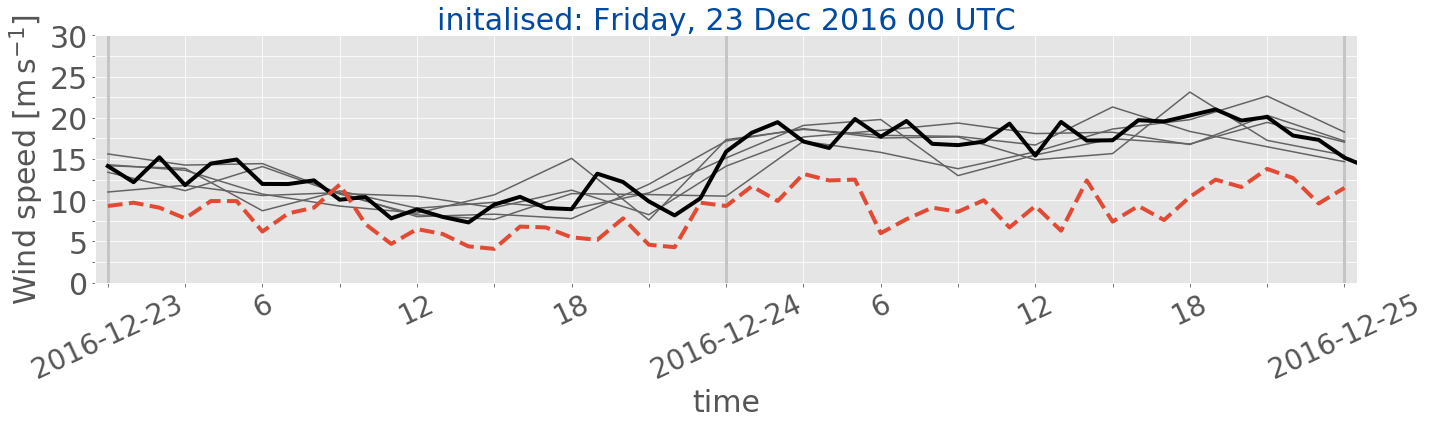
\includegraphics[trim={0.cm 5.cm 0cm 0cm},clip,
		width=\textwidth]{./fig_sfc_ws/20161223_00}
		\caption{}\label{fig:res:sfc_ws23}
	\end{subfigure}
	%
	\begin{subfigure}[b]{0.49\textwidth}
		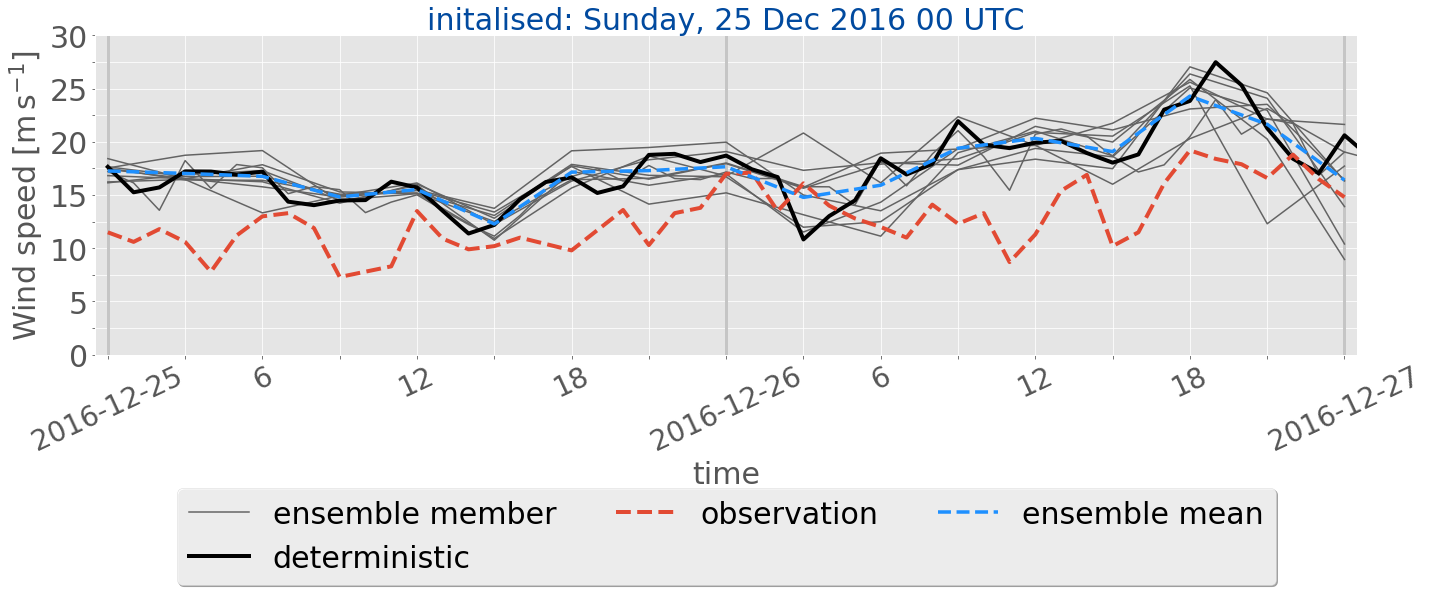
\includegraphics[trim={0.cm 5.cm 0cm 0cm},clip,
		width=\textwidth]{./fig_sfc_ws/20161225_00}
		\caption{}\label{fig:res:sfc_ws25}
	\end{subfigure}
	% sfc precip
	\begin{subfigure}[b]{0.49\textwidth}
		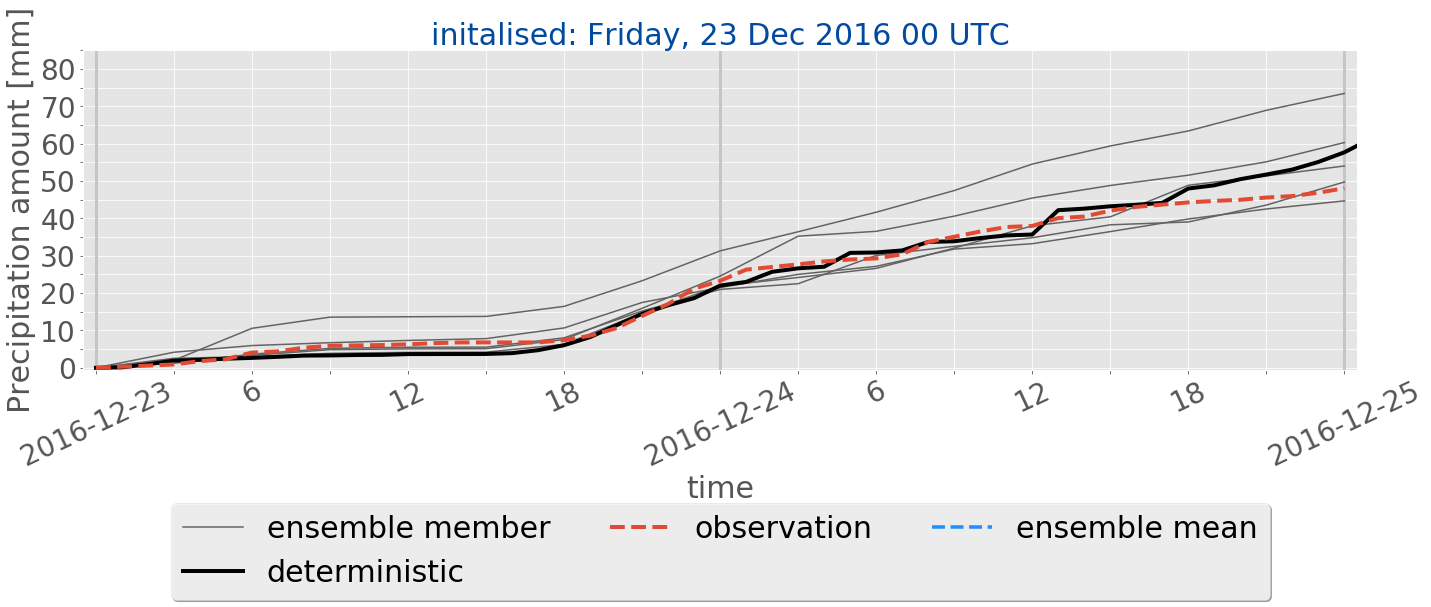
\includegraphics[trim={0.cm 3.6cm 0cm 0cm},clip,
		width=\textwidth]{./fig_sfc_precip/20161223_00}
		\caption{}\label{fig:res:sfc_precip23}
	\end{subfigure}
	%
	\begin{subfigure}[b]{0.49\textwidth}
		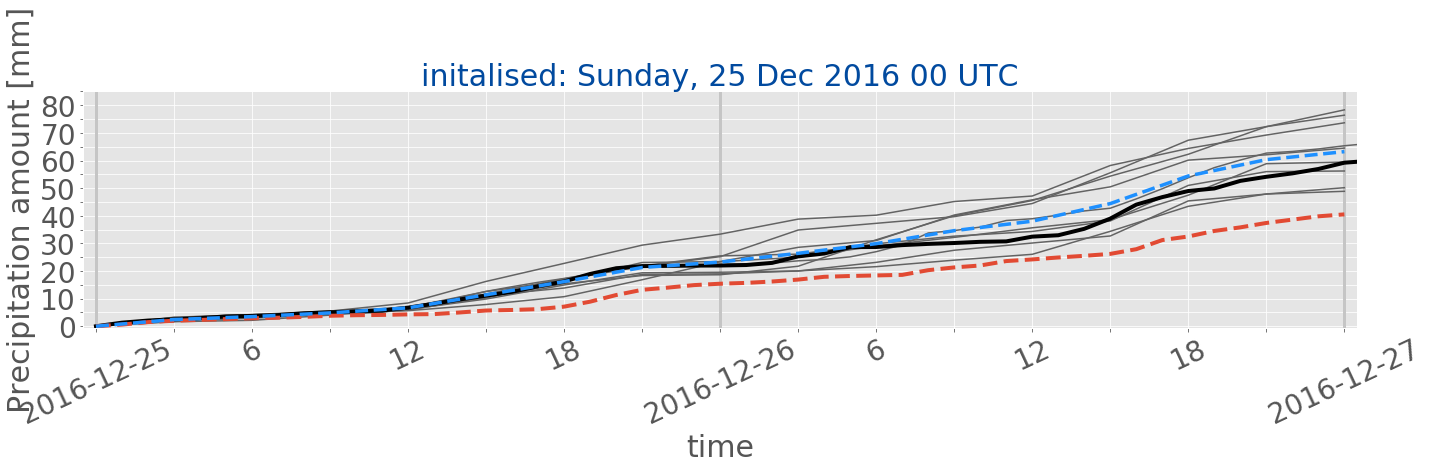
\includegraphics[trim={0.cm 3.6cm 0cm 0cm},clip,
		width=\textwidth]{./fig_sfc_precip/20161225_00}
		\caption{}\label{fig:res:sfc_precip25}
	\end{subfigure}
	
	% label
	\begin{subfigure}[b]{\textwidth}
		\centering
		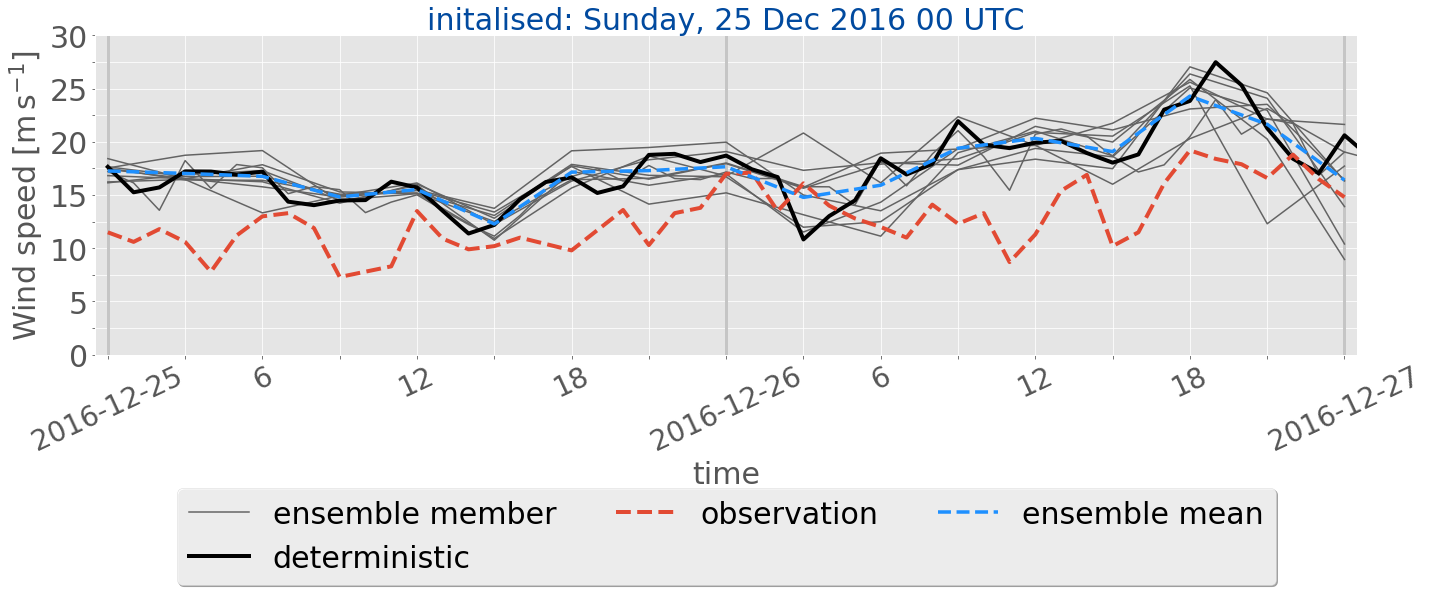
\includegraphics[trim={5.5cm 0cm 5.cm 17.2cm},clip,
		width=0.8\textwidth]{./fig_sfc_ws/20161225_00}
	\end{subfigure}
	\caption{\SI{48}{\hour} surface observations and MEPS ensemble forecasts initialised on the \SI{23}{\dec} at \SI{0}{\UTC} (left column, \protect\subref{fig:res:sfc_pres23}, \protect\subref{fig:res:sfc_temp23}, \protect\subref{fig:res:sfc_wd23}, \protect\subref{fig:res:sfc_ws23}, \protect\subref{fig:res:sfc_precip23}), and on \SI{25}{\dec} at \SI{0}{\UTC} (right column, \protect\subref{fig:res:sfc_pres25}, \protect\subref{fig:res:sfc_temp25}, \protect\subref{fig:res:sfc_wd25}, \protect\subref{fig:res:sfc_ws25}, \protect\subref{fig:res:sfc_precip25}) as well as \SI{26}{\dec} (\protect\subref{fig:res:sfc_pres26}, \protect\subref{fig:res:sfc_temp26}, \protect\subref{fig:res:sfc_wd26}, \protect\subref{fig:res:sfc_ws26}, \protect\subref{fig:res:sfc_precip26}). Line representation according to the label. Upper to low panel: sea level pressure, \SI{2}{\metre} air temperature, \SI{10}{\metre} wind direction and speed, and precipitation amount. }\label{fig:res:sfc_obs_meps}
	%
\end{figure}
\begin{figure}[H]\ContinuedFloat
	\centering
	% sfc pressure
	\begin{subfigure}[b]{0.49\textwidth}
		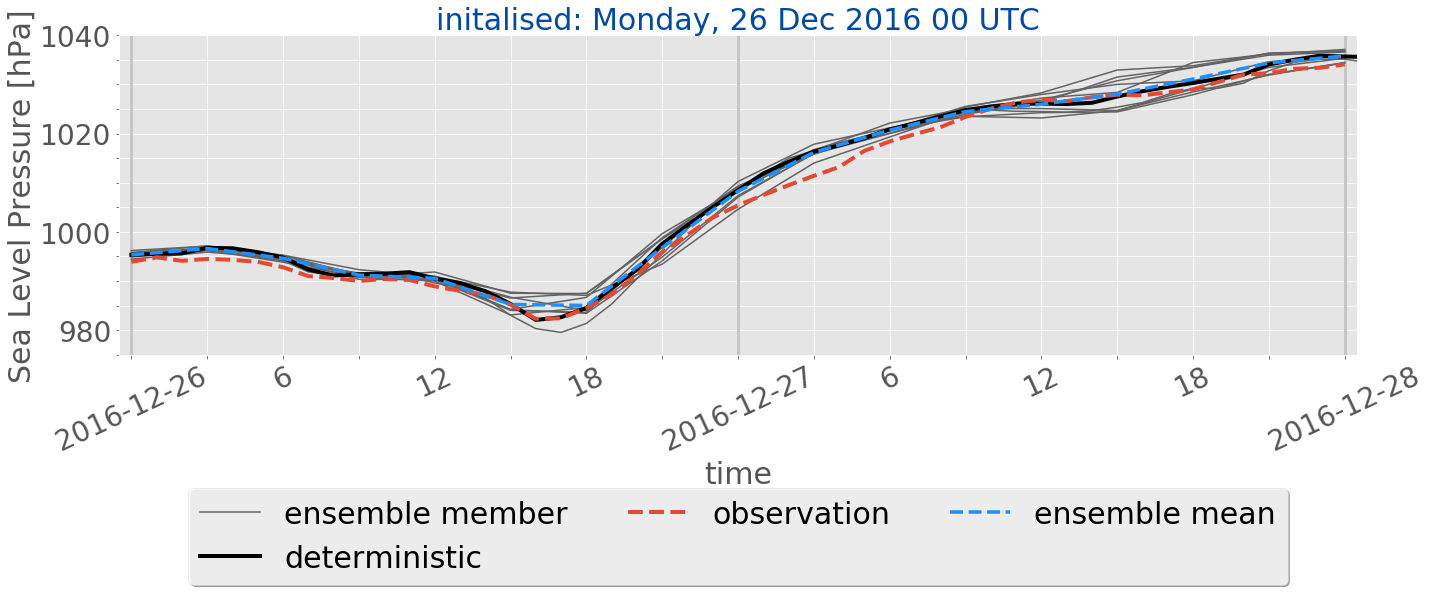
\includegraphics[trim={0.cm 5.cm 0cm 0cm},clip,
		width=\textwidth]{./fig_sfc_pressure/20161226_00}
		\caption{}\label{fig:res:sfc_pres26}
	\end{subfigure}
	
	% sfc temp
	\begin{subfigure}[b]{0.49\textwidth}
		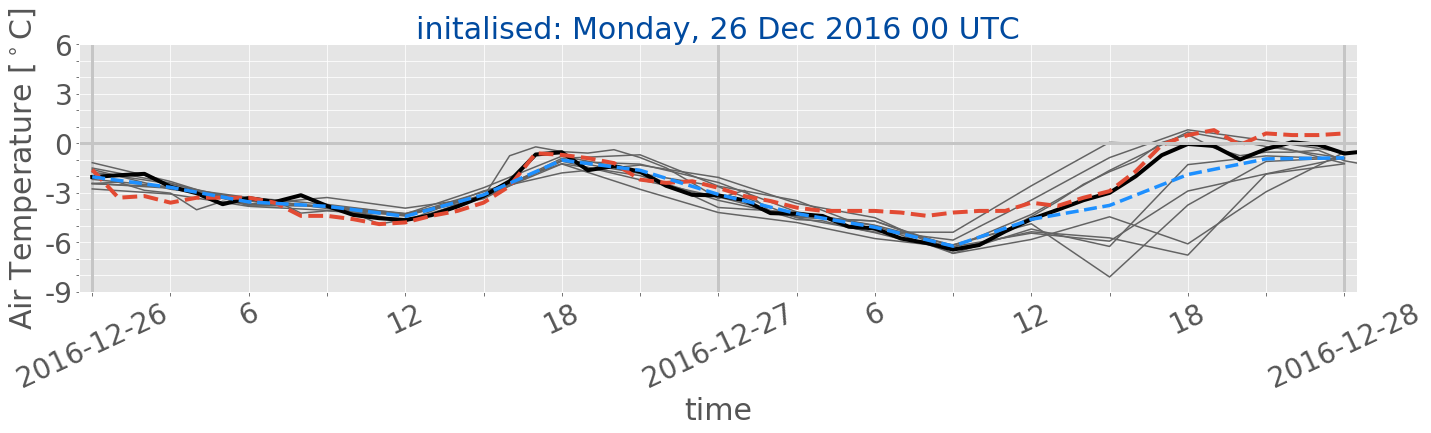
\includegraphics[trim={0.cm 5.cm 0cm 0cm},clip,
		width=\textwidth]{./fig_sfc_temp/20161226_00}
		\caption{}\label{fig:res:sfc_temp26}
	\end{subfigure}
	
	% sfc wd
	\begin{subfigure}[b]{0.49\textwidth}
		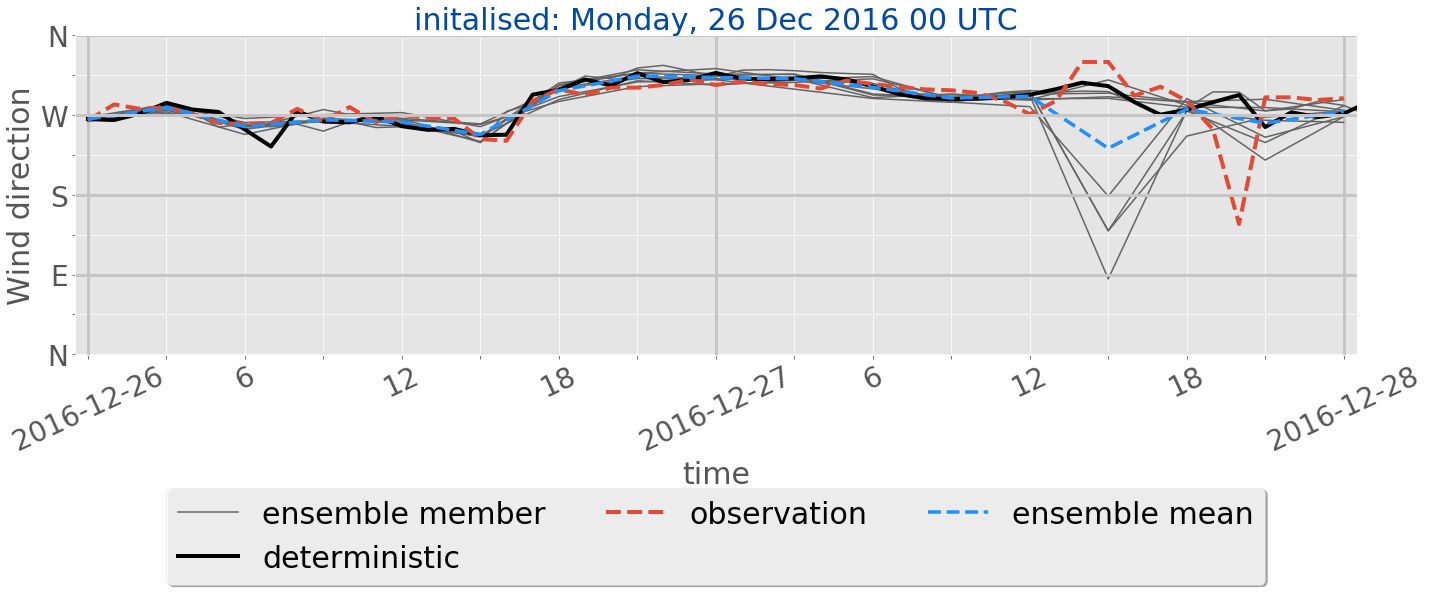
\includegraphics[trim={0.cm 5.cm 0cm 0cm},clip,
		width=\textwidth]{./fig_sfc_wd/20161226_00}
		\caption{}\label{fig:res:sfc_wd26}
	\end{subfigure}
	
	% sfc ws
	\begin{subfigure}[b]{0.49\textwidth}
		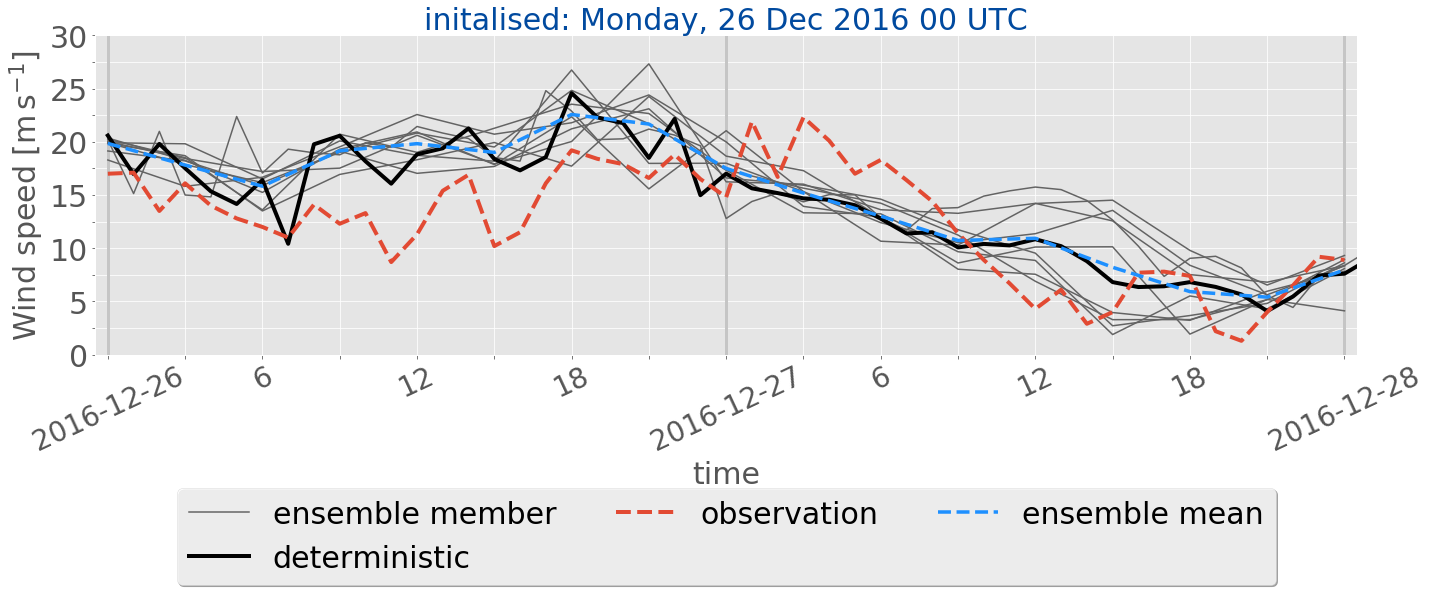
\includegraphics[trim={0.cm 5.cm 0cm 0cm},clip,
		width=\textwidth]{./fig_sfc_ws/20161226_00}
		\caption{}\label{fig:res:sfc_ws26}
	\end{subfigure}
	
	% sfc precip
	\begin{subfigure}[b]{0.49\textwidth}
		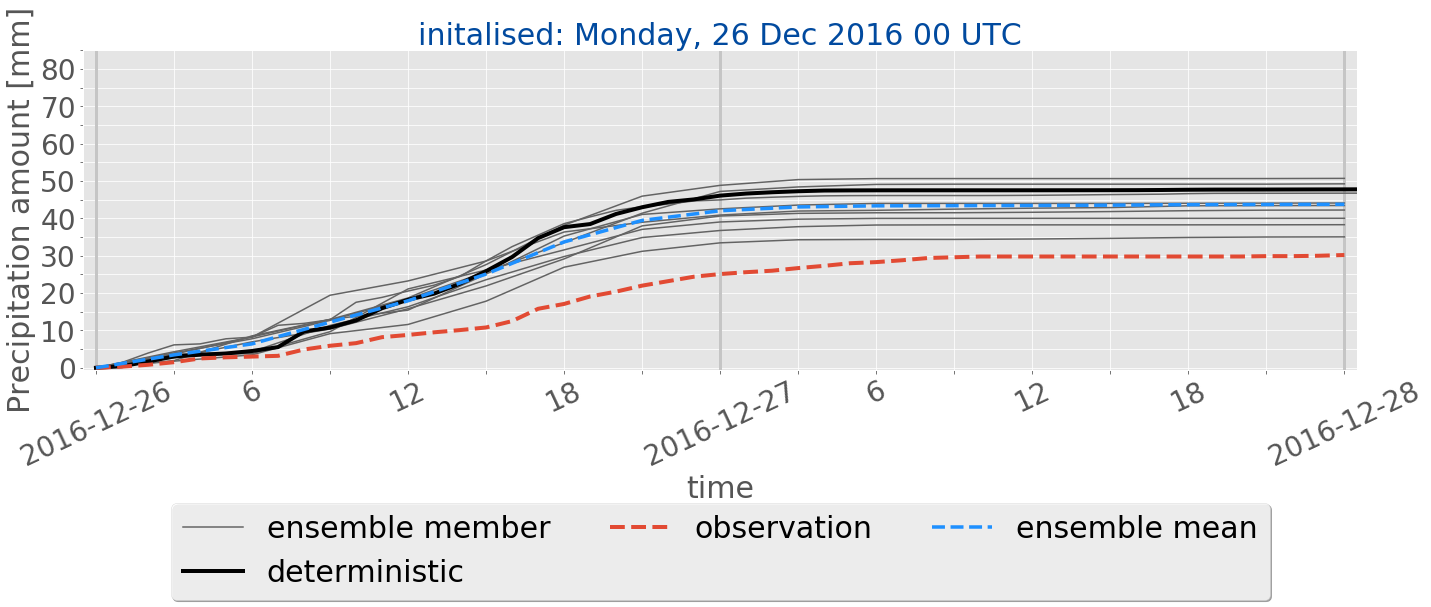
\includegraphics[trim={0.cm 3.6cm 0cm 0cm},clip,
		width=\textwidth]{./fig_sfc_precip/20161226_00}
		\caption{}\label{fig:res:sfc_precip26}
	\end{subfigure}
	
	% label
	\begin{subfigure}[b]{\textwidth}
		\centering
		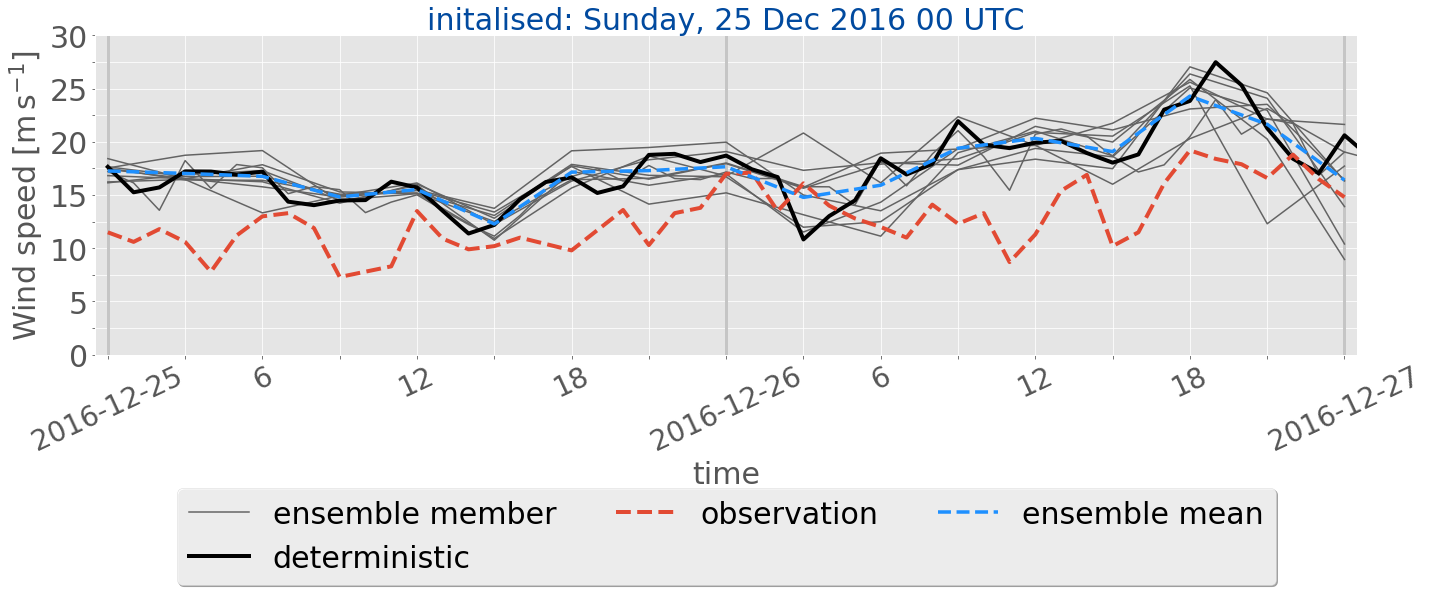
\includegraphics[trim={5.5cm 0cm 5.cm 17.2cm},clip,
		width=0.8\textwidth]{./fig_sfc_ws/20161225_00}
	\end{subfigure}
	\caption{\textit{(Continued from previous page.)} }
\end{figure}
%%%%%%%%%%%%%%%%%%%%%%%%%%%%%%%%%%%%%%%%%%%%%%
%\\
\noindent
\\
As the cyclone is advected to the north-east, closer into the Norwegian Sea, a wind change can be seen in the analysis map from ECMWF (\Cref{fig:GP23}). First west wind and later south-west wind was associated with the low-pressure system. The MEPS forecast and observations in \Cref{fig:res:sfc_wd23} and \subref{fig:res:sfc_ws23} indicate a wind change from west to south with a slight decrease in wind speed.
\\
On \SI{23}{\dec}, the evolution of the occlusion is also observed by an increase in precipitation. Before \SI{18}{\UTC} the surface accumulation shows light precipitation (\Cref{fig:res:sfc_precip23}). During the transition of the occluded front, the observed surface accumulation increases which is associated to continuous, heavy precipitation.  shown in \Cref{fig:res:sfc_precip23}.
\\
\\
Similar patterns as on \SI{23}{\dec} were seen for the transition of the occluded front on \SI{26}{\dec} in the ECMWF analysis \Cref{fig:DT26} and \ref{fig:GP26}. In this case the low-pressure system was located north of Morø and Romsdal in the Norwegian Sea. In the morning the cyclone is located east of Iceland and in the course of the day it moves closer to the coast of Norway. Before landfall at \SI{16}{\UTC}, a pressure decrease occurs (\Cref{fig:res:sfc_pres26}). During the development of the occluded front, the sea level pressure reaches its lowest point of \SI{985}{\hPa} and increases afterwards during the dissipation of the Christmas storm. Pressure, temperature, and wind changes for the occlusion transition were already forecasted for initialisations on \SI{25}{\dec} (\Cref{fig:res:sfc_pres25}, \subref{fig:res:sfc_temp25}, \subref{fig:res:sfc_wd25}, \subref{fig:res:sfc_ws25}), only wind speed and precipitation seem not to agree with the observations at Haukeliseter. \textcolor{red}{Kicki: see Discussion point?}
\\
Since the cyclone was surrounded by colder air (south of the low-pressure system in \Cref{fig:DT26}), first a drop and then an increase of temperature were observed and forecasted by MEPS (\Cref{fig:res:sfc_temp26}). An indication of the occlusion evolution is also visible in the \SI{10}{\metre} wind observations and forecasts. 
On \SI{26}{\dec} at \SI{0}{\UTC}, the low pressure system is east of Iceland (not shown \textcolor{red}{Double check}), moving closer into the Norwegian Sea by \SI{12}{\UTC} (\Cref{fig:DT26} and \ref{fig:GP26}). 
Surface west winds are associated to the cyclone in the Norwegian Sea, and impinging on the West coast of Norway \Cref{fig:GP26}. The wind measurement and MEPS forecast in \Cref{fig:res:sfc_wd26} and \ref{fig:res:sfc_ws26}, show a gentle west breeze of up to \SI{17}{\mPs} at Haukeliseter before \SI{12}{\UTC}.
The centre of the occluded front is located over Norway at \SI{18}{\UTC}, and the pronounced surface pressure gradient, in \Cref{fig:GP26_18}, indicate an increase in surface wind with a north-west wind direction. During this transition of the occlusion, the wind direction changes to north-west with higher observed wind speed up to \SI{20}{\mPs} (\Cref{fig:res:sfc_wd26} and \ref{fig:res:sfc_ws26}). 
\\
Precipitation is continuing throughout the day, with light to moderate precipitation before the occlusion transition seen in \Cref{fig:res:sfc_precip26}. Heavy precipitation around \SI{16}{\UTC} is followed by moderate to light precipitation on \SI{26}{\dec}. 
\\
%%%%%%% image liquid obs particle %%%%%%%%%%%%%%%%
\begin{figure}[t]
	\centering
	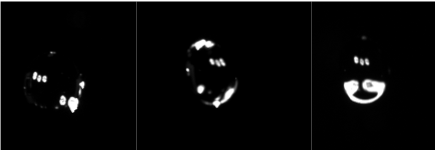
\includegraphics[%trim={45.cm 30.cm 13cm 35cm},clip,
	width=0.8\textwidth]{./MASC_obs/Masc_obs_liquid_2512}
	\caption{MASC images of falling water drops observed on \SI{25}{\dec} at \SI{17}{\UTC} from three different angles. Not all parts of the liquid sphere are equally illuminated.}\label{fig:res:obs_masc}
\end{figure}
%%%%%%%%%%%%%%%%%%%%%%%%%%%%%%%%%%%%%%%%%%%%%%
\\
While on \num{23} and \SI{26}{\dec} the precipitation was associated with a transition/landfall of an occluded front, the \SI{25}{\dec} was marked by the transition of a warm sector. The ECMWF analysis shows a ridging at the dynamic tropopause (\Cref{fig:DT25}). The surface cyclone core is south east of Iceland in \Cref{fig:DT25} with two associated frontal boundaries. While the warm front is approaching the west coast, the cold front is north-west of Great Britain. In \Cref{fig:GP25}, the cold fronts tail moved into lower latitudes, following the slowdown of the cold front, leading to a stationary frontal boundary. Furthermore, the mid-latitude jet is aligned along the surface frontal boundaries (\Cref{fig:DT25_00}), while the Haukeliseter site is located below the the midlatitudal jet (\Cref{fig:GP25_00}). %This leads to rising motion at the surface.
\\
Neither pressure nor wind observations and forecasts indicate the evolution of any frontal boundary. The only indication of a transition could be seen in the increase of temperature at \SI{11}{\UTC} until \SI{21}{\UTC} (\Cref{fig:res:sfc_temp25}). In \Cref{fig:res:sfc_wd25}, a small wind change from west to north-west is observed by the wind mast at \SI{10}{\UTC}, which is not forecasted by MEPS, it rather estimated strong west winds.
\\
In \Cref{fig:res:obs_masc}, particle images taken by the MASC are available, during the transition of the warm sector. Without the images taken around \SI{17}{\UTC} it would only be possible to verify that liquid precipitation occurred with the optical precipiation detectors at the Haukeliseter site. Together with the increase in surface temperature (\Cref{fig:res:sfc_temp25}) it can be concluded the warm sector of the Christmas 2016 event passed by the measurement site.
\textcolor{red}{Should I include the DIANA analysis maps? But I dont know what the meteorologists are using to produce them? ECMWF?}
%
%%%%%%% image scatter obs ret %%%%%%%%%%%%%%%%
\begin{figure}[t!]
	\centering
	% sfc pressure
	\begin{subfigure}[b]{0.49\textwidth}
		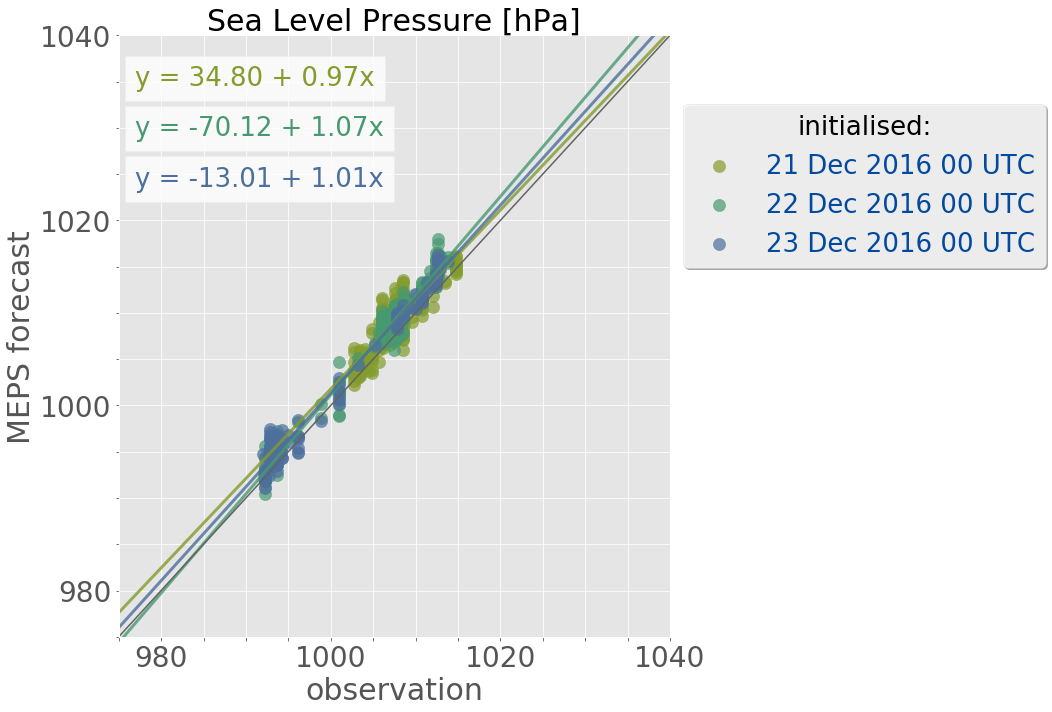
\includegraphics[trim={0.cm 0cm 12.5cm 0cm},clip,
		width=\textwidth]{./fig_sfc_pressure/obs_model_20161221_23_00}
		\caption{}\label{fig:scat:pres2123}
	\end{subfigure}
	%
	\begin{subfigure}[b]{0.49\textwidth}
		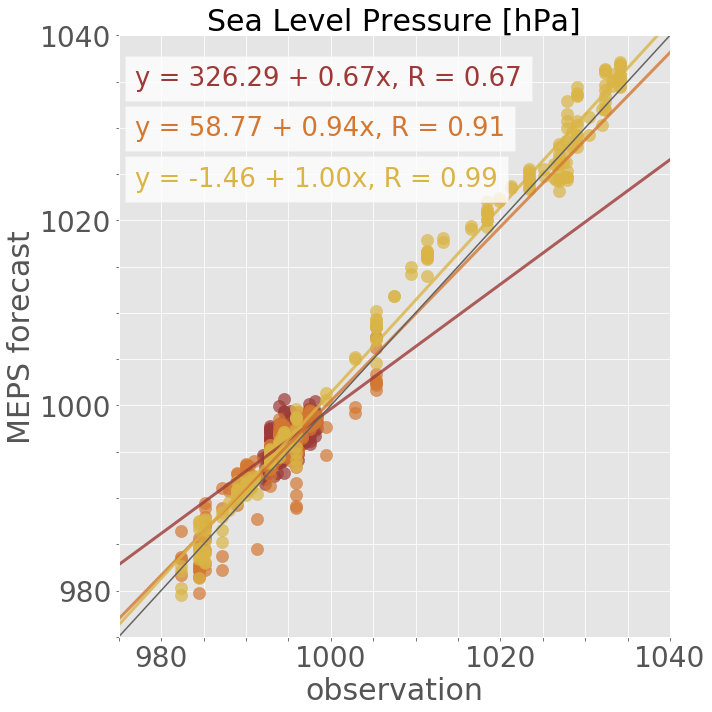
\includegraphics[trim={0.cm 0cm 12.5cm 0cm},clip,
		width=\textwidth]{./fig_sfc_pressure/obs_model_20161224_26_00}
		\caption{}\label{fig:scat:pres2426}
	\end{subfigure}
	%
	% label
	\begin{subfigure}[b]{0.49\textwidth}
		\centering
		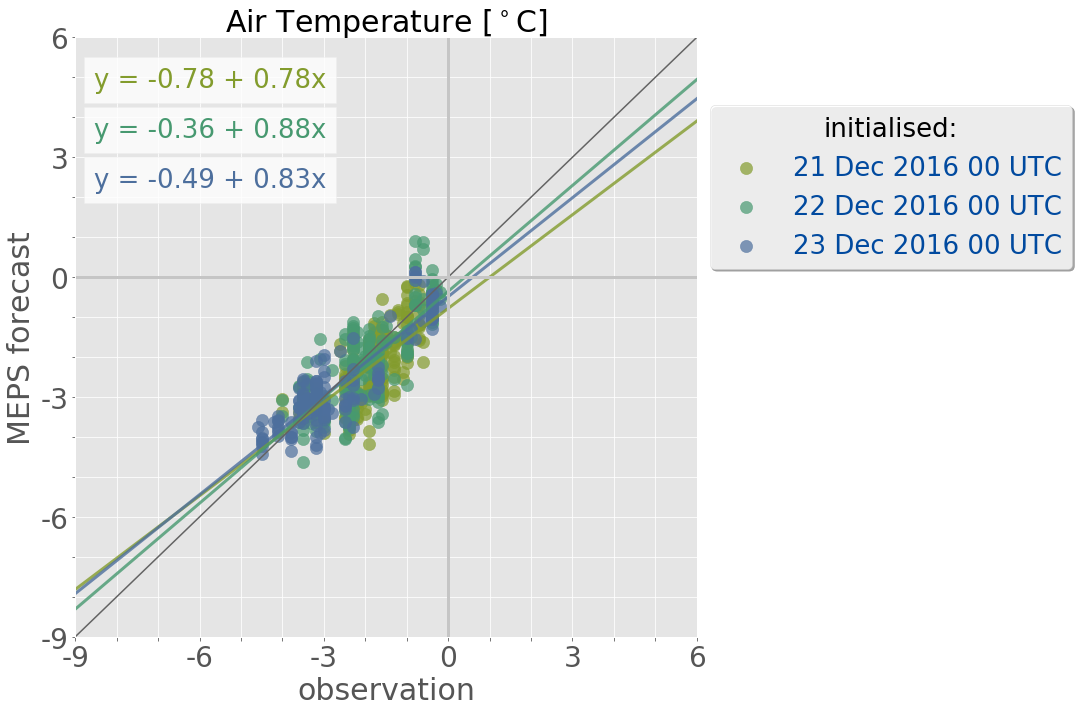
\includegraphics[trim={25.cm 15.5cm 0cm 3.6cm},clip,
		width=0.8\textwidth]{./fig_sfc_temp/obs_model_20161221_23_00}
	\end{subfigure}
	\begin{subfigure}[b]{0.49\textwidth}
		\centering
		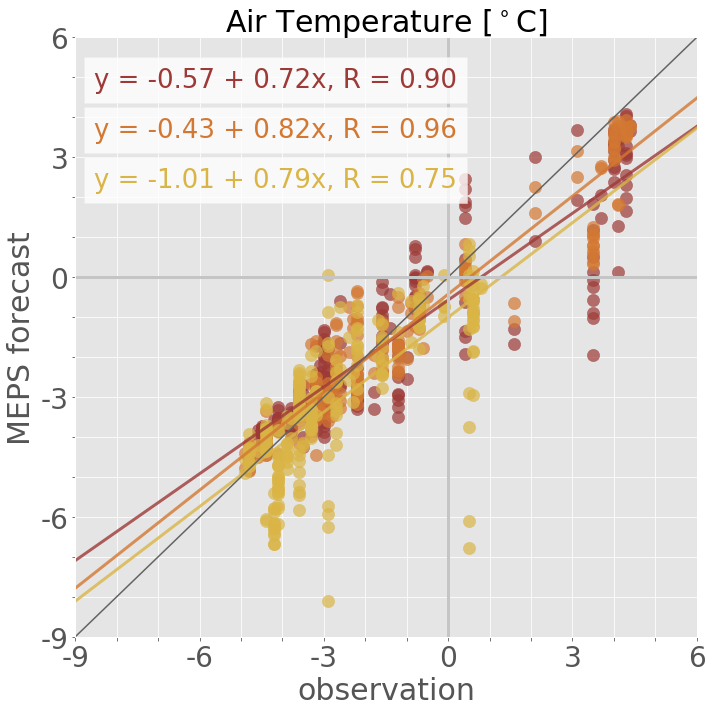
\includegraphics[trim={25.cm 15.5cm 0cm 3.6cm},clip,
		width=0.8\textwidth]{./fig_sfc_temp/obs_model_20161224_26_00}
	\end{subfigure}
	\caption{Sea level pressure [\SI{}{\hPa}] for \SI{48}{\hour} for surface observations and ensemble forecasts initialised for \SIrange{21}{23}{\dec} (left column, \protect\subref{fig:scat:pres2123}, \protect\subref{fig:scat:temp2123}, \protect\subref{fig:scat:wd2123}, \protect\subref{fig:scat:ws2123}, \protect\subref{fig:scat:precip2123}) and  for \num{24} ton \SI{26}{\dec} (right column, \protect\subref{fig:scat:pres2426}, \protect\subref{fig:scat:temp2426}, \protect\subref{fig:scat:wd2426}, \protect\subref{fig:scat:ws2426}, \protect\subref{fig:scat:precip2426}). The \SI{48}{\hour} scatter values indicate each day, according to the colours.  }\label{fig:scat:obs_meps}
\end{figure}
\begin{figure}\ContinuedFloat
	\centering
	%     % sfc temp
	\begin{subfigure}[b]{0.49\textwidth}
		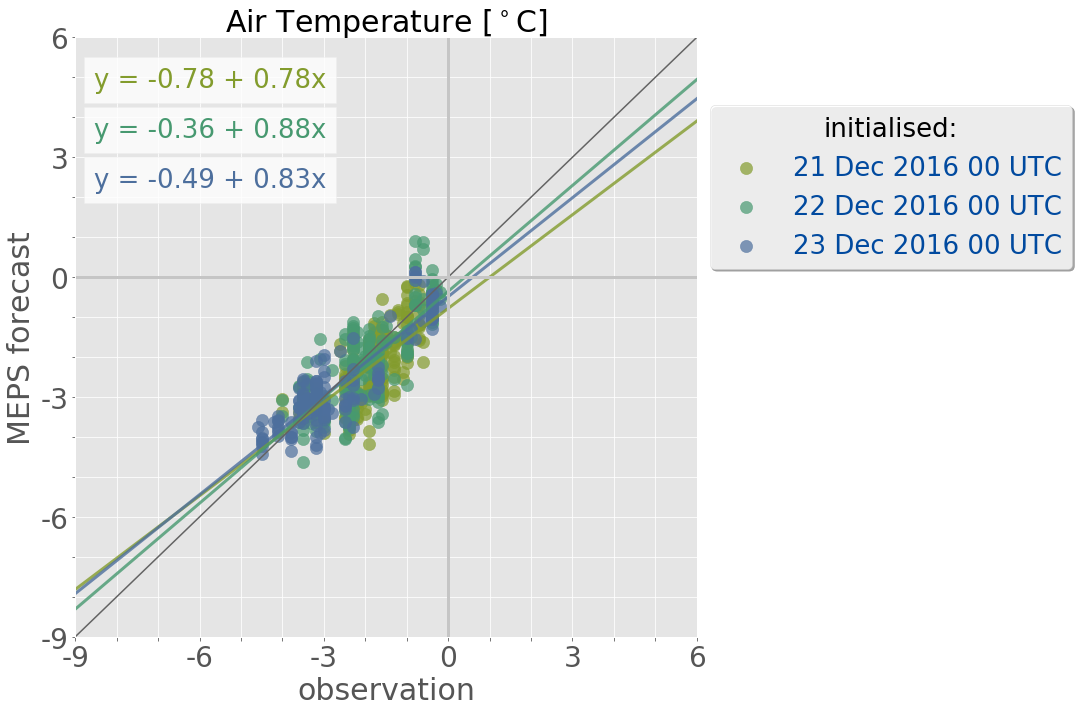
\includegraphics[trim={0.cm 0cm 12.5cm 0cm},clip,
		width=\textwidth]{./fig_sfc_temp/obs_model_20161221_23_00}
		\caption{}\label{fig:scat:temp2123}
	\end{subfigure}
	%
	\begin{subfigure}[b]{0.49\textwidth}
		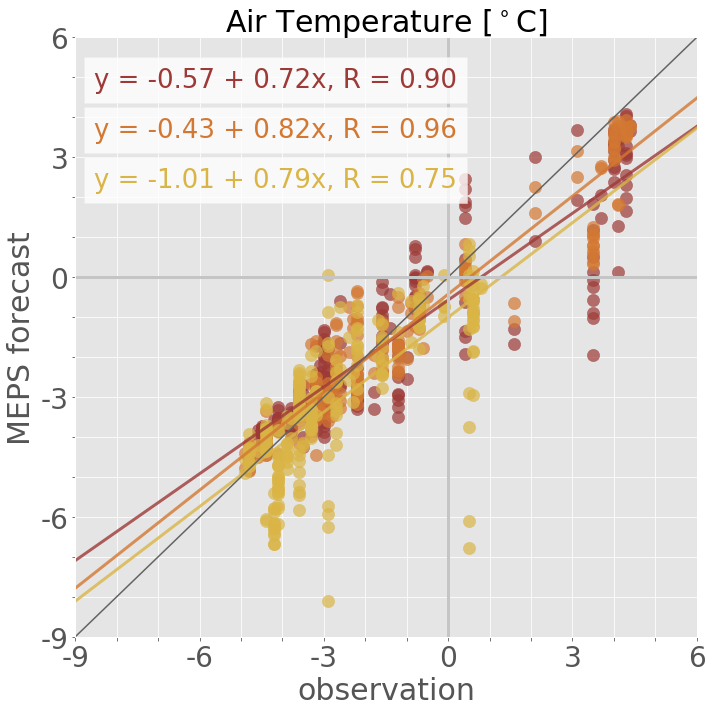
\includegraphics[trim={0.cm 0cm 12.5cm 0cm},clip,
		width=\textwidth]{./fig_sfc_temp/obs_model_20161224_26_00}
		\caption{}\label{fig:scat:temp2426}
	\end{subfigure}
	% 
	% sfc wd
	\begin{subfigure}[b]{0.49\textwidth}
		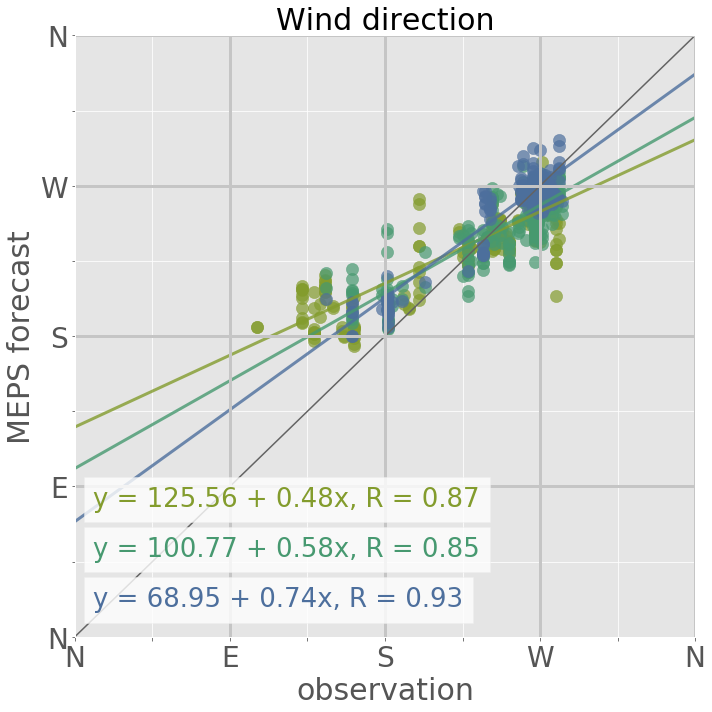
\includegraphics[trim={0.cm 0cm 12.5cm 0cm},clip,
		width=\textwidth]{./fig_sfc_wd/obs_model_20161221_23_00}
		\caption{}\label{fig:scat:wd2123}
	\end{subfigure}
	%
	\begin{subfigure}[b]{0.49\textwidth}
		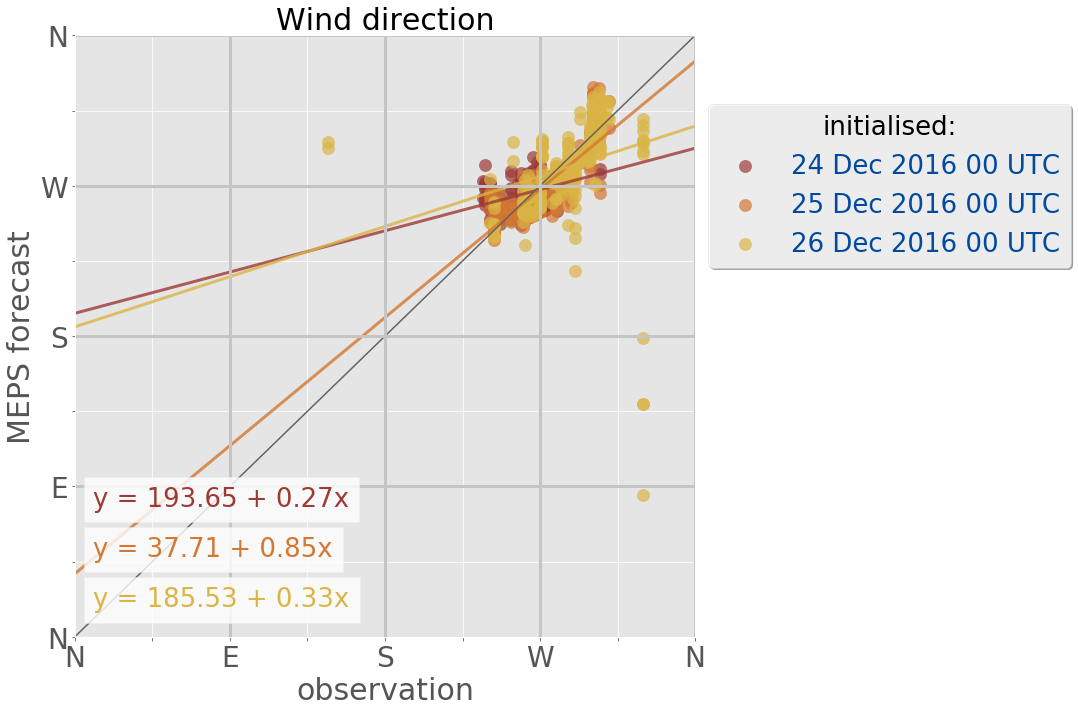
\includegraphics[trim={0.cm 0cm 12.5cm 0cm},clip,
		width=\textwidth]{./fig_sfc_wd/obs_model_20161224_26_00}
		\caption{}\label{fig:scat:wd2426}
	\end{subfigure}
	
	% label
	\begin{subfigure}[b]{0.49\textwidth}
		\centering
		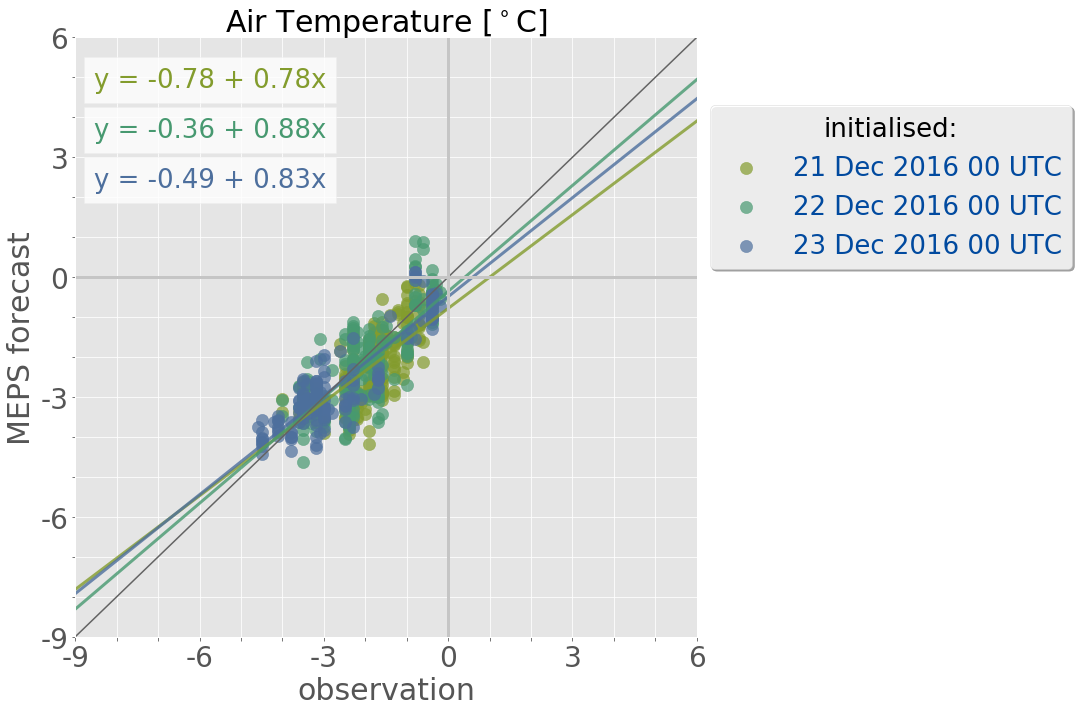
\includegraphics[trim={25.cm 15.5cm 0cm 3.6cm},clip,
		width=0.8\textwidth]{./fig_sfc_temp/obs_model_20161221_23_00}
	\end{subfigure}
	\begin{subfigure}[b]{0.49\textwidth}
		\centering
		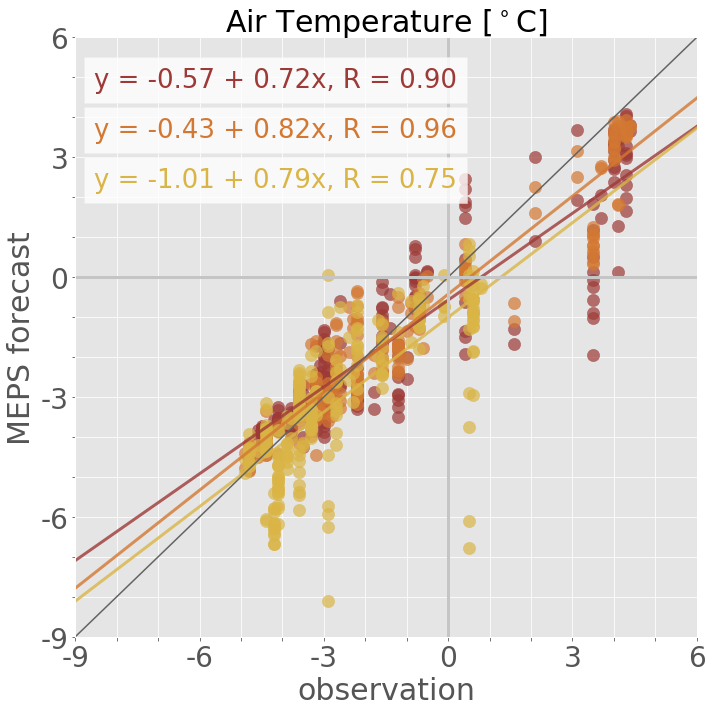
\includegraphics[trim={25.cm 15.5cm 0cm 3.6cm},clip,
		width=0.8\textwidth]{./fig_sfc_temp/obs_model_20161224_26_00}
	\end{subfigure}
	\caption{\textit{(Continued from previous page.)} Upper panel \SI{2}{\metre} air temperature, second panel \SI{10}{\metre} wind direction.}
\end{figure}
\begin{figure}\ContinuedFloat
	% sfc ws
	\begin{subfigure}[b]{0.49\textwidth}
		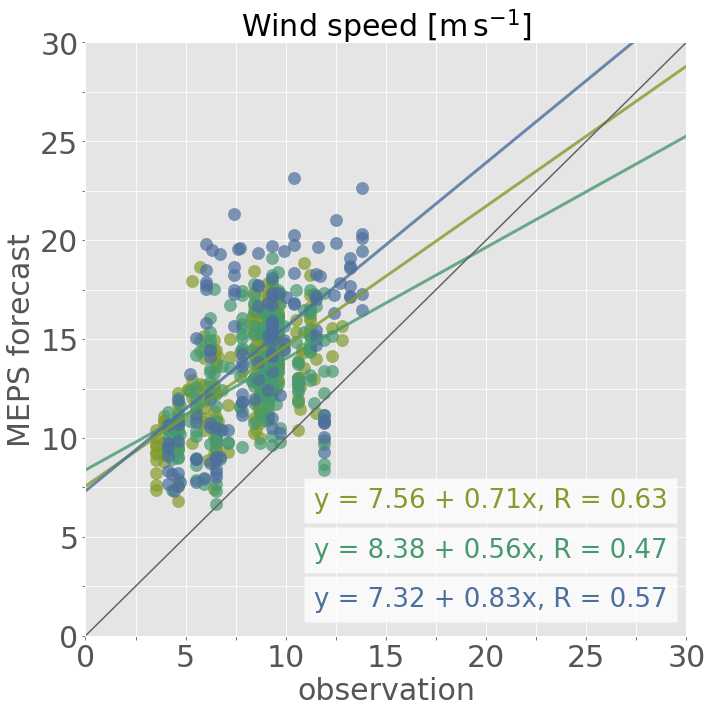
\includegraphics[trim={0.cm 0cm 12.5cm 0cm},clip,
		width=\textwidth]{./fig_sfc_ws/obs_model_20161221_23_00}
		\caption{}\label{fig:scat:ws2123}
	\end{subfigure}
	%
	\begin{subfigure}[b]{0.49\textwidth}
		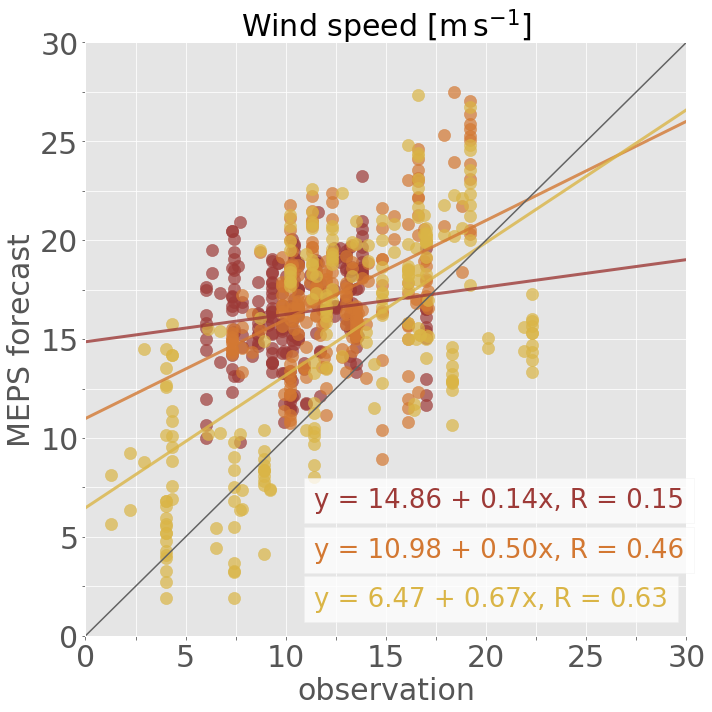
\includegraphics[trim={0.cm 0cm 12.5cm 0cm},clip,
		width=\textwidth]{./fig_sfc_ws/obs_model_20161224_26_00}
		\caption{}\label{fig:scat:ws2426}
	\end{subfigure}
	% sfc precip
	\begin{subfigure}[b]{0.49\textwidth}
		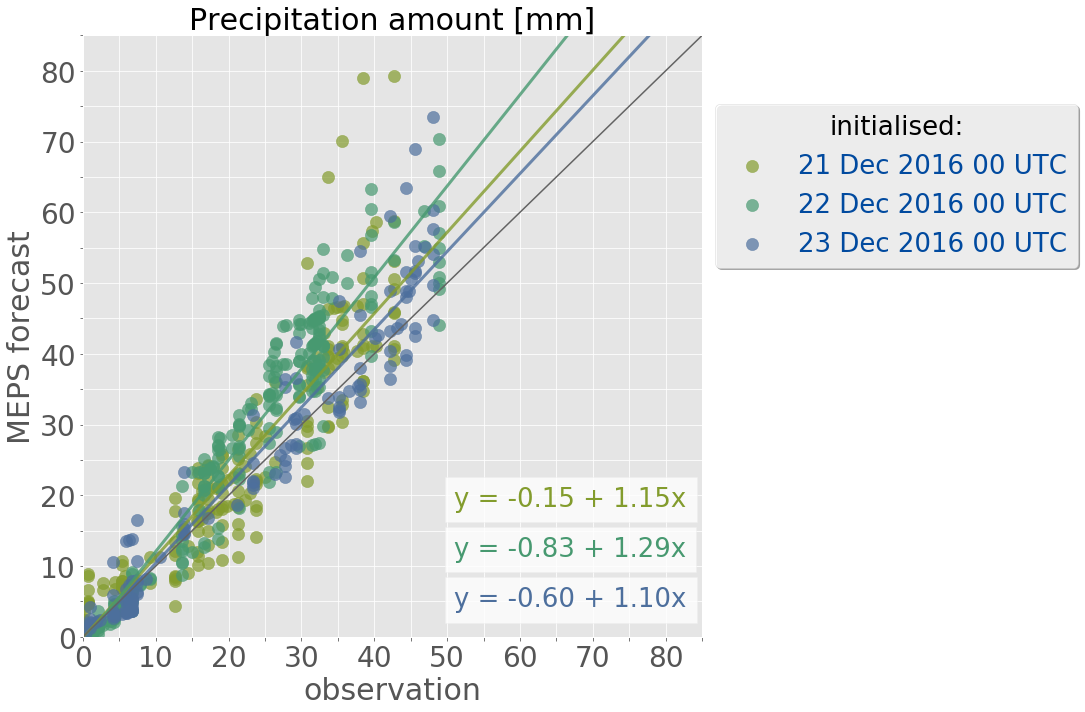
\includegraphics[trim={0.cm 0cm 12.5cm 0cm},clip,
		width=\textwidth]{./fig_sfc_precip/obs_model_20161221_23_00}
		\caption{}\label{fig:scat:precip2123}
	\end{subfigure}
	%
	\begin{subfigure}[b]{0.49\textwidth}
		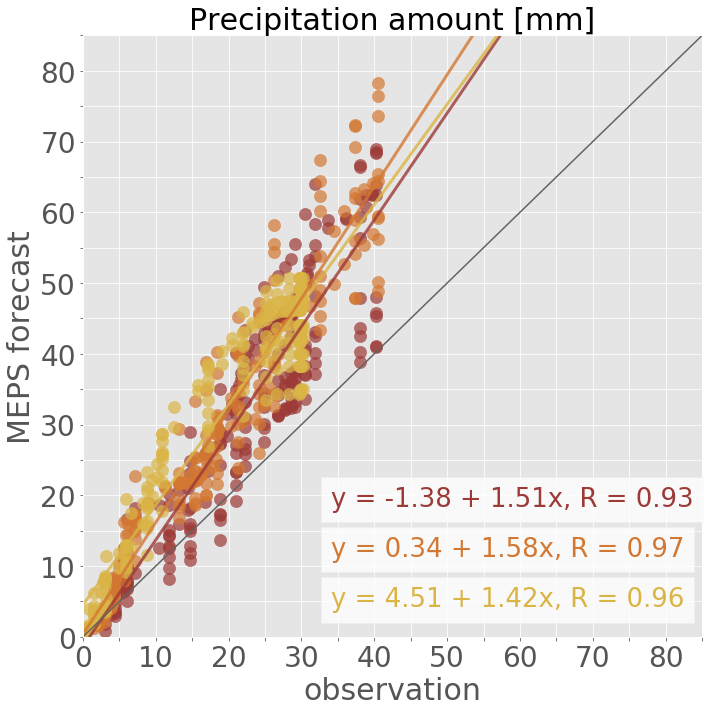
\includegraphics[trim={0.cm 0cm 12.5cm 0cm},clip,
		width=\textwidth]{./fig_sfc_precip/obs_model_20161224_26_00}
		\caption{}\label{fig:scat:precip2426}
	\end{subfigure}
	% label
	\begin{subfigure}[b]{0.49\textwidth}
		\centering
		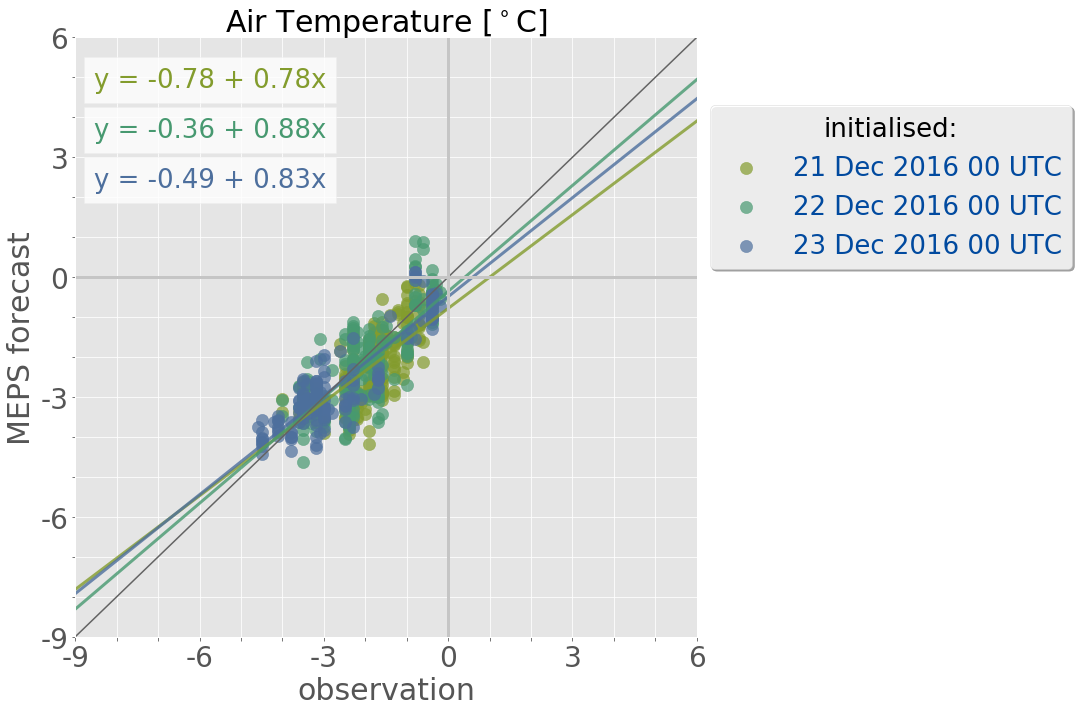
\includegraphics[trim={25.cm 15.5cm 0cm 3.6cm},clip,
		width=0.8\textwidth]{./fig_sfc_temp/obs_model_20161221_23_00}
	\end{subfigure}
	\begin{subfigure}[b]{0.49\textwidth}
		\centering
		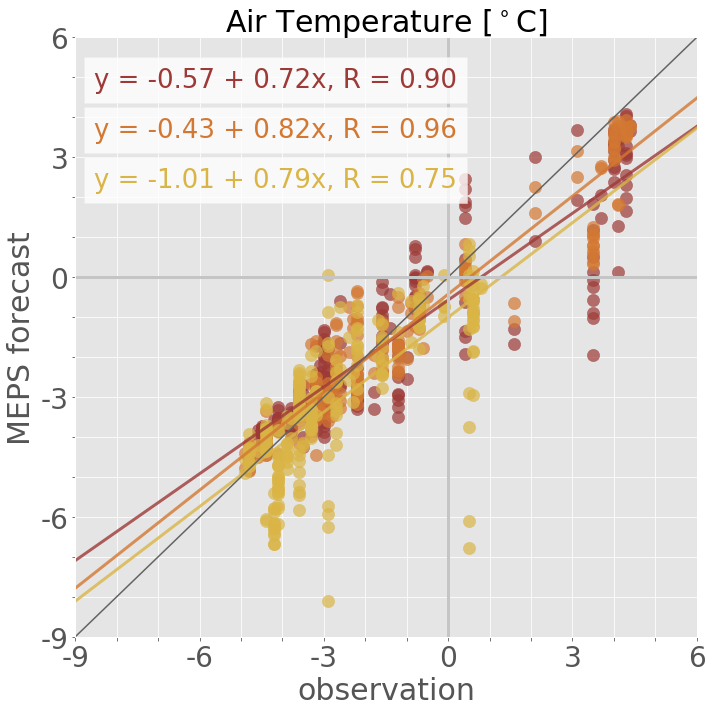
\includegraphics[trim={25.cm 15.5cm 0cm 3.6cm},clip,
		width=0.8\textwidth]{./fig_sfc_temp/obs_model_20161224_26_00}
	\end{subfigure}
	\caption{\textit{(Continued from previous page.)} Upper panel \SI{10}{\metre} wind speed, lower panel surface precipitation amount. }
\end{figure}
%%%%%%%%%%%%%%%%%%%%%%%%%%%%%%%%%%%%%%%%%%%%%%
\\
\\
The comparison between the ECMWF analysis (\Cref{sec:largeScale}) and the observations at the measurement site (\Cref{fig:res:sfc_obs_meps}), that the ensemble member forecast system MEPS covers the prediction of large scale phenomena like occlusions and fronts, as well as liquid precipitation at the surface. \Cref{fig:scat:obs_meps} presents the correlation between the observations and the \SI{48}{\hour} MEPS ensemble forecast. The relation for Haukeliseter observations and the MEPS forecast members is indicated with the regression calculated for each day.
\\
Sea level pressure has the best correlation under all variables. The best agreement is reached on \SI{26}{\dec}, when the Christmas storm hit land and dissipated after the evolution of the occlusion at \SI{16}{\UTC}. \citet{dahlgren_comparison_2013} showed an improvement of sea level pressure forecast for AROME, by including large scale boundary conditions for ECMWF into the regional model. The observation-model comparison by \citet{dahlgren_comparison_2013} showed an increase of forecast accuracy after \SI{24}{\hour} with the use of pressure mixing. 
Since surface pressure is in good agreement with the observations, it is assumed that the warm front did not pass through Haukeliseter on \SI{25}{\dec} and only the warm sector associated with the 2016 Christmas storm is observed. This shows a quite detailed forecast ability of MEPS, as from the ECMWF analysis, in \Cref{fig:DT25}, it is not quite clear if the warm front could have passed through. To be sure that the warm front did not pass through Haukeliseter, or whether it is a predictive error of MEPS, surface pressure, temperature and wind should be compared to the nearest grid point of the global forecast model ECMWF.
\\
\Cref{fig:scat:temp2426} displays a moderate correlation between observation and the \SI{48}{\hour} MEPS ensemble member forecast system. In general, MEPS underestimates the observed \SI{2}{\metre} air temperature, but MEPS estimated the surface temperature changes at the correct timing for \num{23}, \num{25}, and \SI{26}{\dec}. The previous operational deterministic forecast model AROME-MetCoOp showed a negative bias of \SI{2}{\metre} temperature after winter 2013 with the introduction of AROME-Norway and later AROME-MetCoOp \citep{muller_arome-metcoop:_2017}. 
The mean error for the Norwegian model domain of AROME-MetCoOP estimated by \citet{muller_arome-metcoop:_2017} is smaller than \SI{1.8}{\kelvin} for the surface temperature in December 2014. In contrast, \Cref{fig:bias:temp} shows warm and cold biases for \num{23} and \SI{26}{\dec}, respectively. On \SI{25}{\dec}, during the warm sector a negative bias was observed, underestimating the temperature when compared to the observation.  The forecasts for \num{23}, \num{25}, and \SI{26}{\dec} show calculated mean absolute error values (\Cref{eq:MAE}) of up to \SIlist{0.61;0.77;1.44}{\kelvin} in \Cref{fig:bias_MAE}. The new ensemble forecast system MEPS shows a reduction of mean errors for the Christmas 2016 extreme event. 
\\
During the Christmas storm 2016, high wind speeds were observed at the Haukeliseter site (\Cref{fig:scat:ws2123} and \subref{fig:scat:ws2426}).
According to \citet{muller_arome-metcoop:_2017} large wind speeds are significantly better simulated for AROME-MetCoOp compared to ECMWF's forecast for the model domain. The wind speed MEPS forecast in \Cref{fig:res:sfc_ws23}, \subref{fig:res:sfc_ws25}, and \subref{fig:res:sfc_ws26} displays still an overestimation of wind speeds. Furthermore, the correlation of observations and wind in \Cref{fig:scat:ws2123} and \subref{fig:scat:ws2426} show a high overestimation for stronger wind speeds on \num{24} to \SI{26}{\dec} than for \num{21} to \SI{23}{\dec}. The inaccuracy for wind speeds is an already known difficulty in the deterministic version of MEPS \citep{muller_arome-metcoop:_2017}. \citet{muller_arome-metcoop:_2017} presented, that AROME-MetCoOp wind speed prediction agreed better with observations for wind speeds between \SIrange{3}{13}{\mPs} than ECMWF forecasts did, showing the advantage of a high-resolution weather model. Furthermore, with increasing wind speed the forecast accuracy for the Norwegian mean decreases with a mean absolute error below \SI{2}{\mPs} for December 2014 in AROME-MetCoOp.
The mean absolute error for wind speed during the Christmas storm is higher for all days ranging from \SIrange{3}{7}{\mPs}.
During the three days with frontal transitions, the highest mean absolute error of \SI{6.5}{\mPs} occurs during \SI{23}{\dec}. More than three times as high as the monthly averaged value for the Norwegian forecast domain from \citet{muller_arome-metcoop:_2017}. Their study case for February 2015 showed a slight overestimation of ECMWF \SI{10}{\metre} wind compared to the Norwegian AROME-MetCoOp forecast, but still overestimates MEPS the wind.
\textcolor{red}{What could be still a weakness that the model overestimates the wind speed? In \citet{muller_arome-metcoop:_2017}: change from ECOCLIMAP1 because the surface roughness was too low and followed high wind speeds? Is this still the case for MEPS? High wind speeds followed also from wrongly adressed 'permanent snow'. Do not use 'orographi drag' in AROME-MetCoOp, could that lead to the too high estimated wind? When 'canopy drag' was changed saw increase in SBL drag which followed a decrease in wind speed. But AROME-MetCoOp is able to forecast high wind speeds, while ECMWF is not.}
\\
Haukeliseter is a measurement site exposed to high wind speeds \citep{wolff_measurements_2013,wolff_derivation_2015}. The ensemble prediction system MEPS still seems to have issues forecasting the wind speed correctly in mountainous terrain.
%\Cref{fig:res:sfc_obs_meps} indicates that MEPS is able to simulate larger scale phenomena which is probably related to the outer boundary conditions of ECMWF as described by \citet{dahlgren_comparison_2013}.
%In general, surface parameters are predicted well, only wind speed and precipitation accumulation showed overestimation in MEPS. Wind speed forecasts are higher than observations, which is probably related to the presentation of the orography in MEPS. 
A detailed insight to the orographical wind influence will be assessed in \Cref{sec:res:oro_infl}. 
\\
\\
\Cref{fig:res:sfc_precip23}, \subref{fig:res:sfc_precip25}, and \subref{fig:res:sfc_precip26} illustrates the surface precipitation amount observed and predicted by MEPS for Haukeliseter. MEPS overestimation is shown for precipitation when the cyclone intensifies and gets closer to Norway on \num{25} and \SI{26}{\dec}. The surface observations and MEPS predictions in \Cref{fig:scat:precip2123} and \subref{fig:scat:precip2426} also show an overestimate for \num{25} and \SI{26}{\dec}, whereas on \SI{23}{\dec} the surface accumulation is balanced for  predictions up to \SI{30}{\mm}. Any reasons for the overestimation of precipitation accumulation on the ground will be further analysed and discussed in \Cref{sec:sfc_acc}.
\\
\\
Overall, the forecast is best for all variables for initialisations on \SI{23}{\dec} (\Cref{fig:scat:pres2123}, \subref{fig:scat:temp2123}, \subref{fig:scat:wd2123}, \subref{fig:scat:ws2123}). 
The large-scale weather pattern seems to be more predictable on \SI{23}{\dec} than initialisations on \num{25} and \SI{26}{\dec}. \Cref{fig:scat:pres2426}, \subref{fig:scat:temp2426}, \subref{fig:scat:wd2426}, \subref{fig:scat:ws2426} suggest as if MEPS has difficulties predicting the intensification and associated pressure drop of the Christmas 2016 storm at Haukeliseter. The prediction of pressure fits well on all three days (\Cref{fig:scat:pres2123}, \subref{fig:scat:pres2426}) compared to temperature, wind direction, wind speed, and precipitation (\Cref{fig:scat:temp2123,fig:scat:temp2426,fig:scat:wd2123,fig:scat:wd2426,fig:scat:ws2123,fig:scat:ws2426,fig:scat:precip2123,fig:scat:precip2426}). The greatest difficulty has MEPS with the prediction of wind speed during the entire extreme event. The rainfall, however, fit well for \SI{23}{\dec} (\Cref{fig:res:sfc_precip23} and \ref{fig:scat:precip2123}), but MEPS has problems predicting the accumulation of surface precipitation amount correctly for the last days of the 2016 Christmas storm, \num{24} to \SI{26}{\dec} (\Cref{fig:res:sfc_precip25}, \subref{fig:res:sfc_precip26} and \Cref{fig:scat:precip2426}).
\\
\textcolor{red}{
	What is the difference between MESP and MetCoOp? What do we want to assess with perturbed ensemble members?\\
	Overall conclusion: Which day was presented worst/best and relate to large scale synoptics}
%%%%%%%%%%%%%%%%%%%%%%%%%%%%%%%%%%%%%%%%%%%%%%%%%%%%%%%%%%%%%%%%%%%%%%%%%%

%%%%%%%%%%%%%%%%%%%%%%%%%%%%%%%%%%%%%%%%%%%%%%%%%%%%%%%%%%%%%%%%%%%%%%%%%
%%%%%%%% Overestimation of surface snowfall %%%%%%%%%%%%%%
\section{Surface snowfall accumulation}\label{sec:sfc_acc}
%%% image surface accumulation %%%%%%%%%%%%%%%%%%%%%%%%%%%%%%%%%%%%%
\begin{figure}[t!]
	\centering
	% 21/12
	\begin{subfigure}[t]{0.49\textwidth}		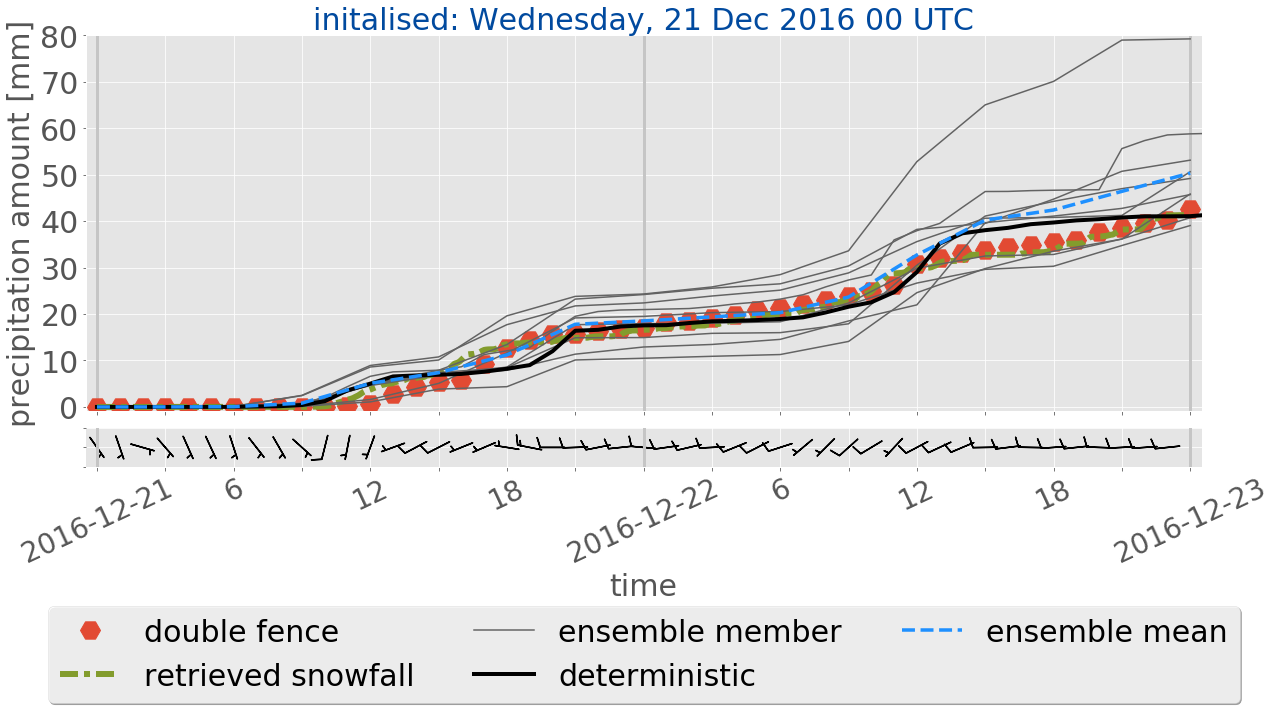
\includegraphics[trim={0.cm 5.2cm 0.cm 0cm},clip,width=\textwidth]{./fig_sfc_acc/acc_wind_20161221_00}
		\caption{}\label{fig:sfc_acc21}
	\end{subfigure}
	% 22/12
	\begin{subfigure}[t]{0.49\textwidth}		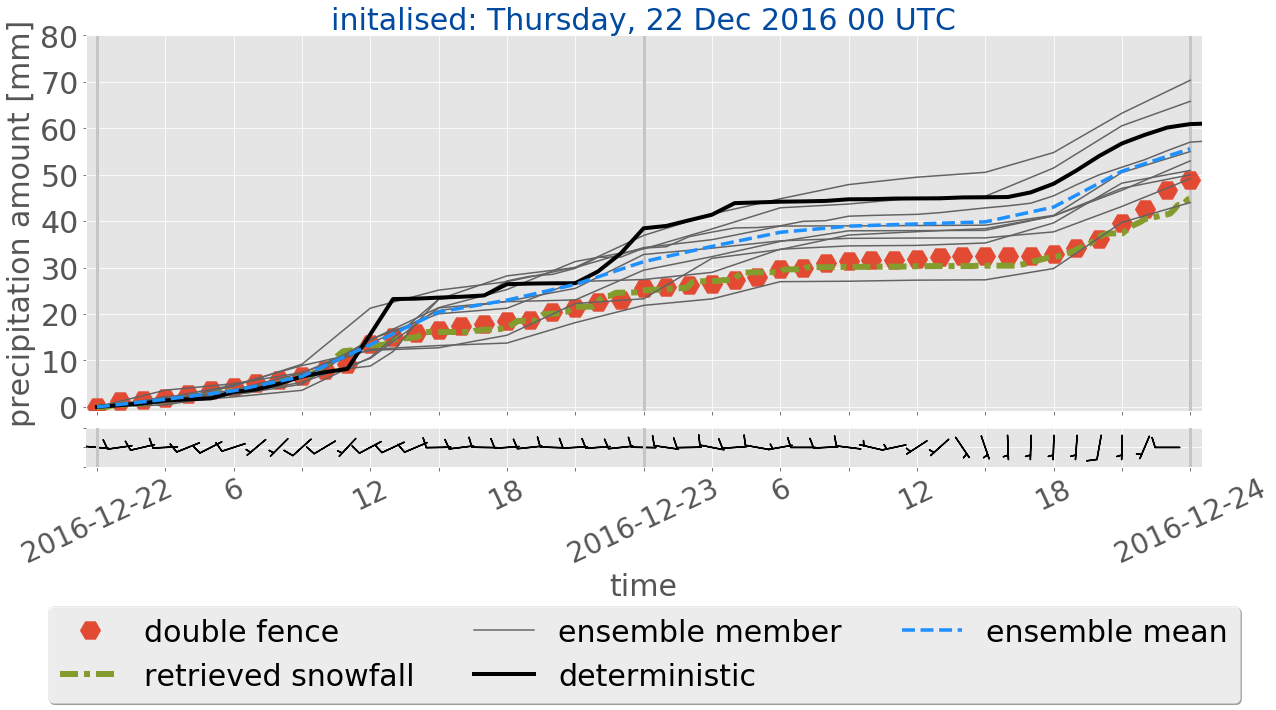
\includegraphics[trim={0.cm 5.2cm 0.cm 0cm},clip,width=\textwidth]{./fig_sfc_acc/acc_wind_20161222_00}
		\caption{}\label{fig:sfc_acc22}
	\end{subfigure}
	%	\end{figure}
	%   \begin{figure}\ContinuedFloat
	% 23/12
	\begin{subfigure}[t]{0.49\textwidth}	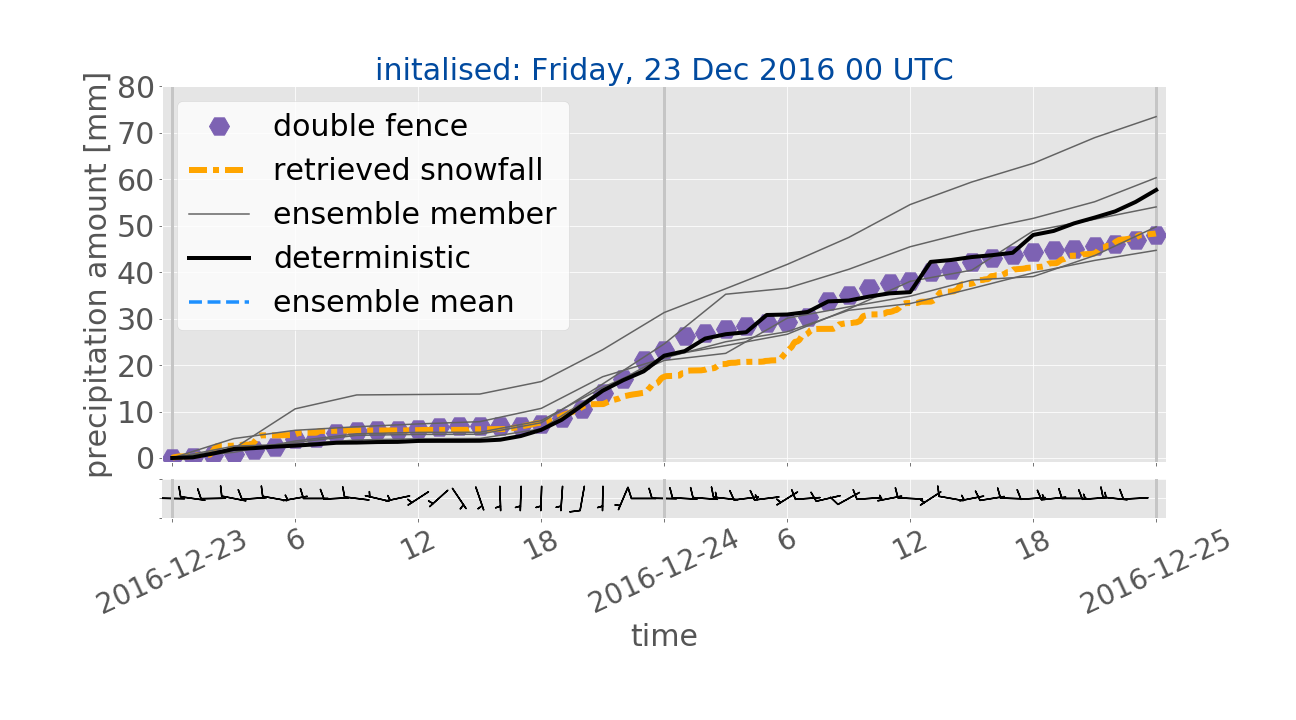
\includegraphics[trim={0.cm 5.2cm 0.cm 0cm},clip,width=\textwidth]{./fig_sfc_acc/acc_wind_20161223_00}
		\caption{}\label{fig:sfc_acc23}
	\end{subfigure}
	% 24/12
	\begin{subfigure}[t]{0.49\textwidth}			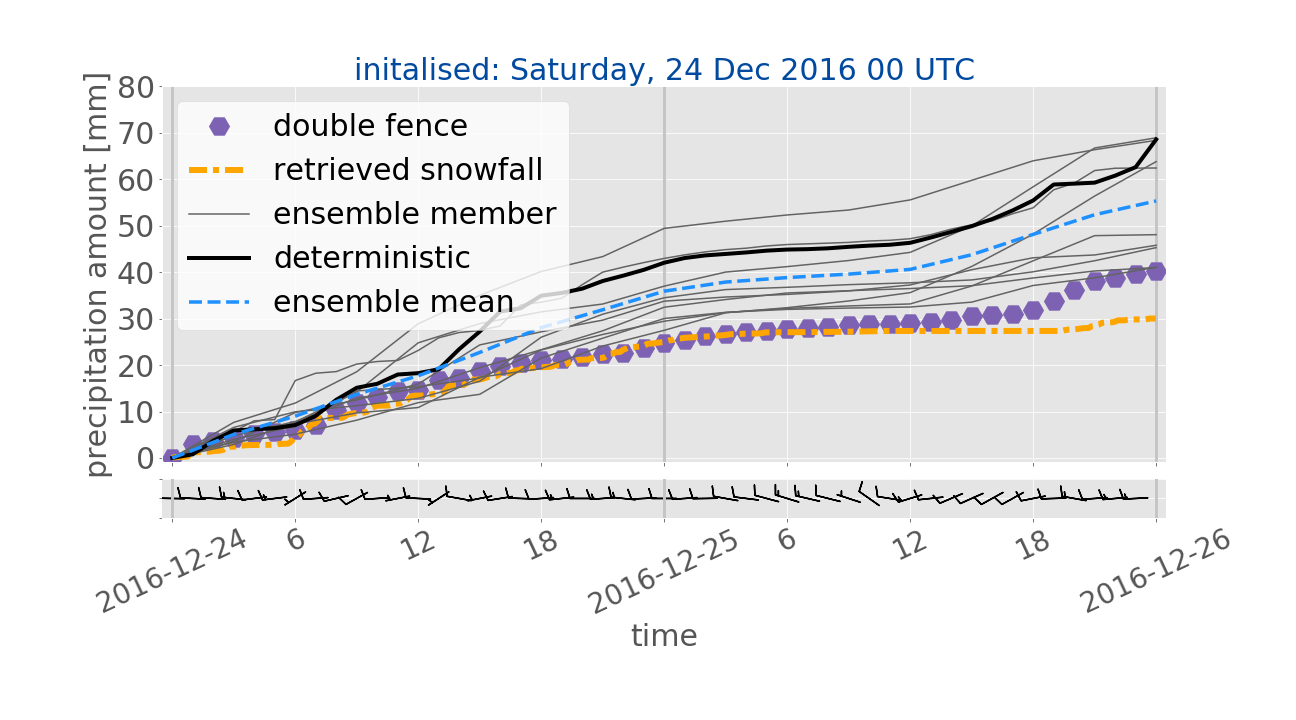
\includegraphics[trim={0.cm 5.2cm 0.cm 0cm},clip,width=\textwidth]{./fig_sfc_acc/acc_wind_20161224_00}
		\caption{}\label{fig:sfc_acc24}
	\end{subfigure}
	% 25/12
	\begin{subfigure}[t]{0.49\textwidth}
		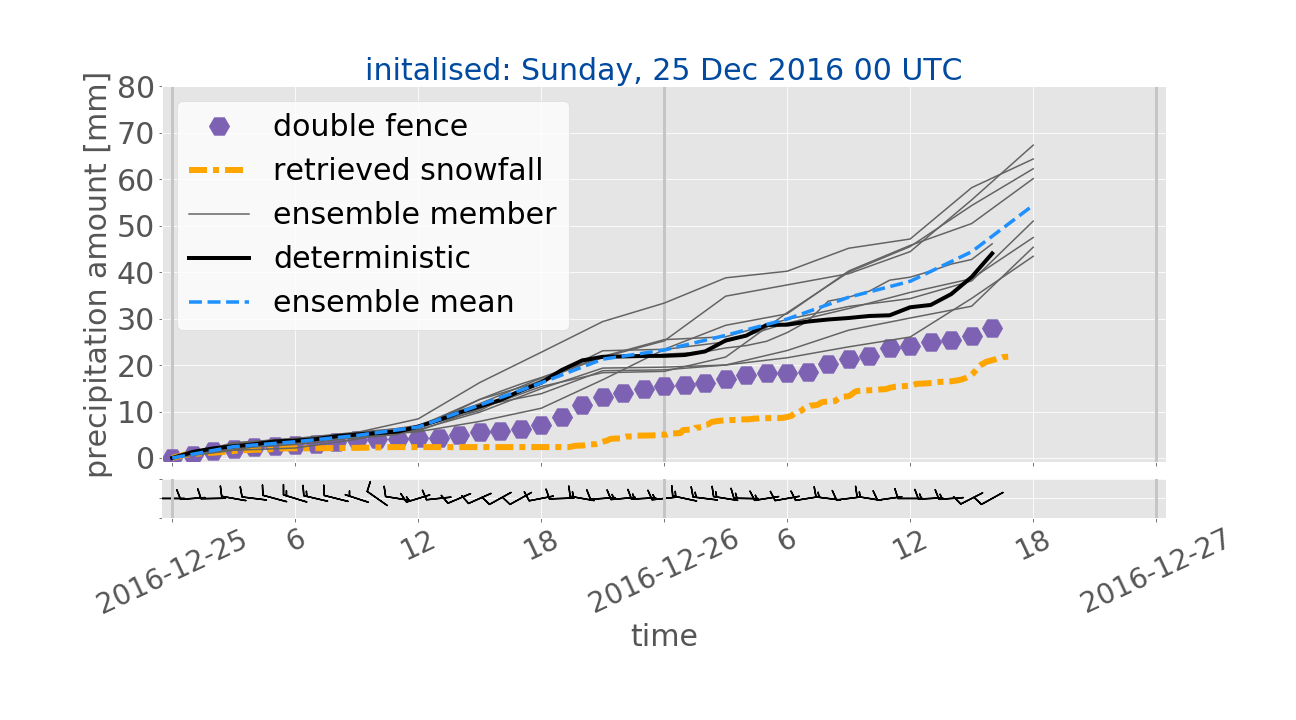
\includegraphics[trim={0.cm 3.6cm 0.cm 0cm},clip,width=\textwidth]{./fig_sfc_acc/acc_wind_20161225_00}
		\caption{}\label{fig:sfc_acc25}
	\end{subfigure}
	% 26/12
	\begin{subfigure}[t]{0.49\textwidth}	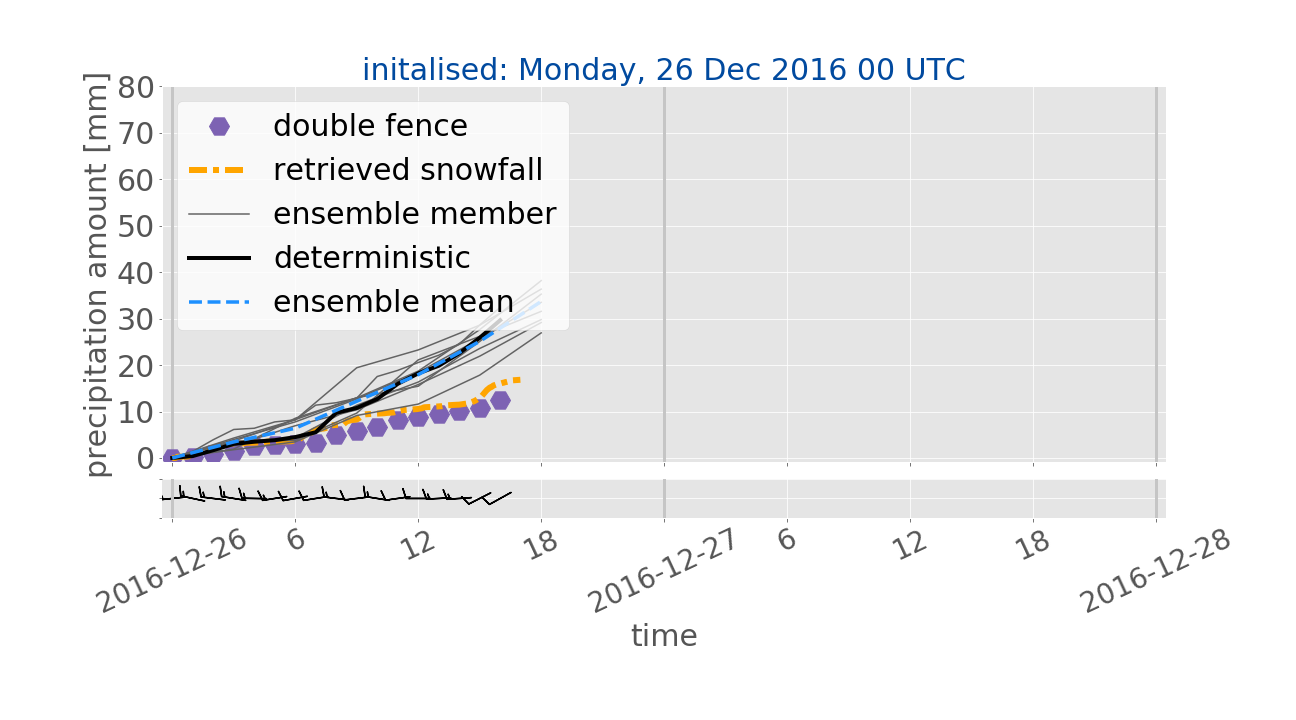
\includegraphics[trim={0.cm 3.6cm 0.cm 0cm},clip,width=\textwidth]{./fig_sfc_acc/acc_wind_20161226_00}
		\caption{}\label{fig:sfc_acc26}
	\end{subfigure}
	
	% label
	\begin{subfigure}[t]{\textwidth}
		\centering
		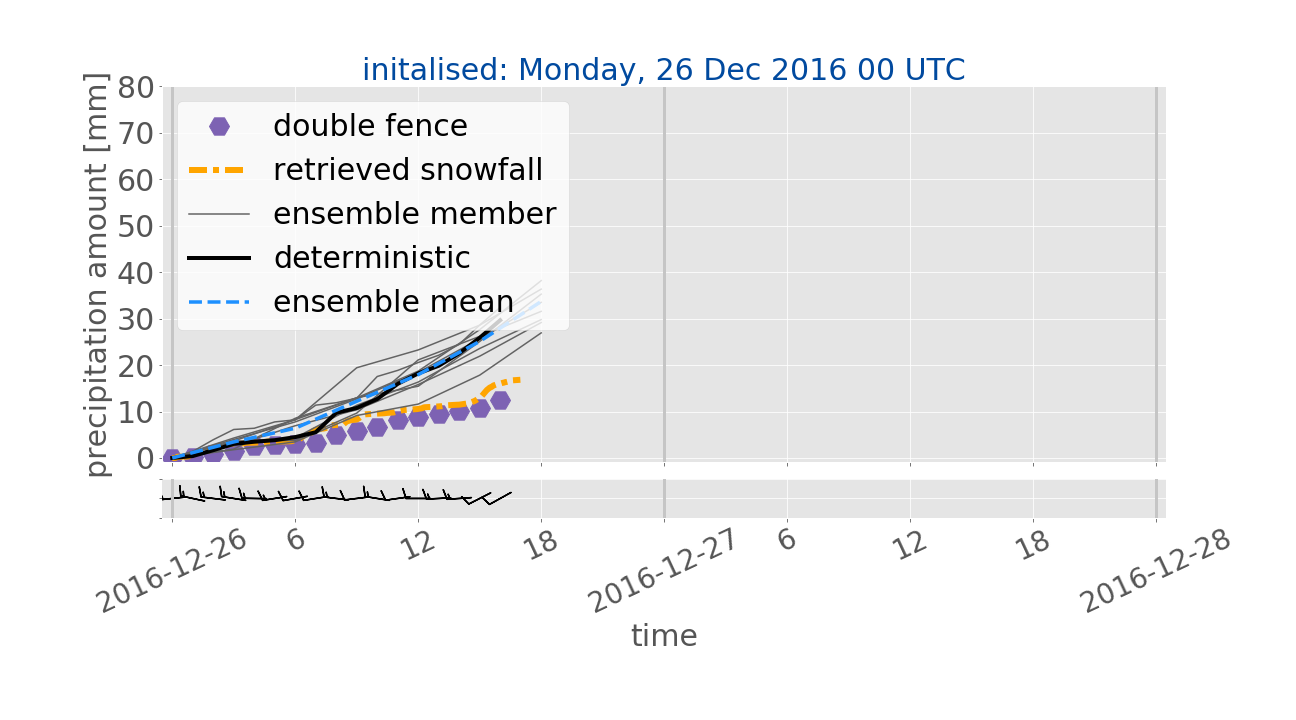
\includegraphics[trim={1.2cm 0cm 1.1cm 21.4cm},clip,width=0.8\textwidth]{./fig_sfc_acc/acc_wind_20161226_00}
	\end{subfigure}
	\caption{\SI{48}{\hour} surface snowfall accumulation for \num{21} to \SI{26}{\dec} (\protect\subref{fig:sfc_acc21}  \protect\subref{fig:sfc_acc26}). Representing the values from the double fence in red, hexagons; optimal estimation retrieval output at snow layer height \SI{400}{\metre} in dash-dotted green; and ensemble member deterministic forecast, initialised at \SI{00}{\UTC} in black and its nine perturbed ensemble members in grey. The ensemble mean of all ten members is shown in dashed blue. Underneath are the associated last hour \SI{10}{\minute} average wind from the weather mast at \SI{10}{\metre} height. }\label{fig:sfc_acc}
\end{figure}
%%%%%%%%%%%%%%%%%%%%%%%%%%%%%%%%%%%%%%%%%%%%%%%%%%%%%%%%%%%%%%%%%%%%%%%%%%
One approach of this study is to see if observed surface accumulation was correctly predicted by the regional weather model MEPS. Precipitation amount at the surface are shown in \Cref{fig:sfc_acc}. The figures are representing the observed and forecasted surface precipitation accumulation in \SI{}{\mm} over \SI{48}{\hour}. Accumulation, measured by the double fence are presented as red hexagons. Minutely retrieved surface snowfall amount in dash-dotted green. The ten \SI{48}{\hour} forecast ensemble members are lines in black and grey, the deterministic and its perturbed ensemble members, respectively. The blue dashed line shows the ensemble mean of all ten members. Since the deterministic and the first ensemble member are having values every hour and the other perturbed members only every three hours, shows the ensemble mean the precipitation amount at \SI{0}{\hour}, \SI{3}{\hour}, $\ldots$, \SI{21}{\hour}, \SI{24}{\hour}, $\ldots$, \SI{48}{\hour} forecast time. When too few ensemble members were present, like on \SI{23}{\dec}, no ensemble mean is calculated (\Cref{fig:sfc_acc23}). 
Underneath is the associated \SI{10}{\minute} average wind of the last hour from the \SI{10}{\metre} weather mast at Haukeliseter, to see if surface accumulation observations may be influenced by wind. 
\\
\Cref{fig:sfc_acc21,fig:sfc_acc22,fig:sfc_acc23} show in general a better agreement between observations and forecast for \SI{48}{\hour} forecasts initialised on \num{21} to \SI{23}{\dec} at \SI{0}{\UTC}. The spread of the ensemble members around the control run fit better to the observations as well than initialisations on \num{24} to \SI{26}{\dec}. 
During these days intensifies the low-pressure system and gets closer advected to the Norwegian coast and influencing the local weather in Norway (\Cref{ch:weather_ana}). \Cref{fig:sfc_acc24,fig:sfc_acc25,fig:sfc_acc26} indicates a larger estimated surface precipitation amount for all ten ensemble members than observed at the measurement site between \num{24} to \SI{26}{\dec}. 
\\ 
\\
The correlation between double fence observation and ensemble forecast is presented in \Cref{fig:scat:pres2123} and \subref{fig:scat:pres2426}. Showing a better agreement between \num{21} to \SI{23}{\dec} than initialisation on \num{24} to \SI{26}{\dec}. On \num{21} to \SI{23}{\dec} is the slope of the regression relatively close to unity, indicating a good agreement between the ensemble forecast and the observations by the double fence.
The largest disagreement between surface observations and forecasts is seen on \SI{25}{\dec} with a positive bias up to \SI{17}{\mm} (\Cref{fig:bias:precip}). The mean absolute error is not larger than \SI{13}{\mm} for the first three days and increases with intensification of the storm up to \SI{19}{\mm} on \SI{24}{\dec}.
\\
Initialisations on \SI{24}{\dec} indicate an overestimation of the deterministic surface snowfall prediction already after \SI{13}{\hour} forecast time. The deterministic forecast in solid black is much higher and increases faster than the observations. In \Cref{fig:sfc_acc24} at \SI{16}{\UTC} a higher value of approximately \SI{15}{\mm} can be seen when compared to the surface measurements. This difference remains almost constantly over the forecast time. Furthermore, all ensemble members seem to overestimate the surface accumulation after \SI{24}{\hour} prediction time. 
\\
Since the MEPS performance was better on the previous days one might assume that the double fence measurement is influenced by surface winds. It shows in \Cref{fig:sfc_acc24} that the \SI{10}{\minute} average wind at \SI{13}{\UTC} increases from \SI{5}{\mPs} to \SI{10}{\mPs} (see also \Cref{fig:res:sfc_ws24}). \citet[][unpublished]{wolff_wmo_2018} states that the double fence gauge is influenced by wind, but accumulation measurement errors occur rather at higher wind speeds larger than \SI{20}{\mPs}. It is therefore assumed that the measurements from the double fence are correct and MEPS had rather a forecasting issue.
\\
While the cyclone gets more advected to Norway increases the forecast inaccuracy of the surface precipitation. 
On \SI{25}{\dec} the miscalculation of the precipitation amount is associated with the warm sector evolution at Haukeliseter (\Cref{sec:res:large_scale_sfc}). Afterwards follows the model the same path as the double fence observations, but higher. The \SI{25}{\dec} indicates a good spread between the ensemble members and the deterministic forecast, while on \SI{24}{\dec} the ensemble members were not spread symmetrically around the deterministic forecast. 
\\
An overestimation of the surface accumulation is also observed on \SI{26}{\dec}. While the large-scale analysis indicates the development of an occlusion after \SI{15}{\UTC} (\Cref{fig:DT26}, \ref{fig:GP26}) seems the overestimation to occur after \SI{12}{\hour} forecast time in \Cref{fig:sfc_acc26}. Again, all ensemble members seem to follow the course of the double fence accumulation, but larger. 
\\
Whereas the spread between the ensemble members is large in the beginning of \SI{24}{\dec} is the variability between the members narrow for \num{25} and \SI{26}{\dec}. The variability between the ensemble member can be compared with a box-whisker plot. A box-whisker-plot shows the time evolution of the distribution of the precipitation amount made of ten ensemble members up to \SI{48}{\hour}. Since some ensemble member do not have forecast values every hour provides the box-whisker-plot in \Cref{fig:boxplot} information every \SI{3}{\hour}. The red line shows the ensemble mean of all ten members and shows if the distribution is skewed. The short light green horizontal line is showing the median, wide vertical box represents the 25th and 75th percentiles, and minimum and maximum values are indicated by the vertical lines, whiskers.
\\
%%% image surface accumulation %%%%%%%%%%%%%%%%%%%%%%%%%%%%%%%%%%%%%
\begin{figure}[h!]
	\centering
	\begin{subfigure}[b]{\textwidth}
		\centering
		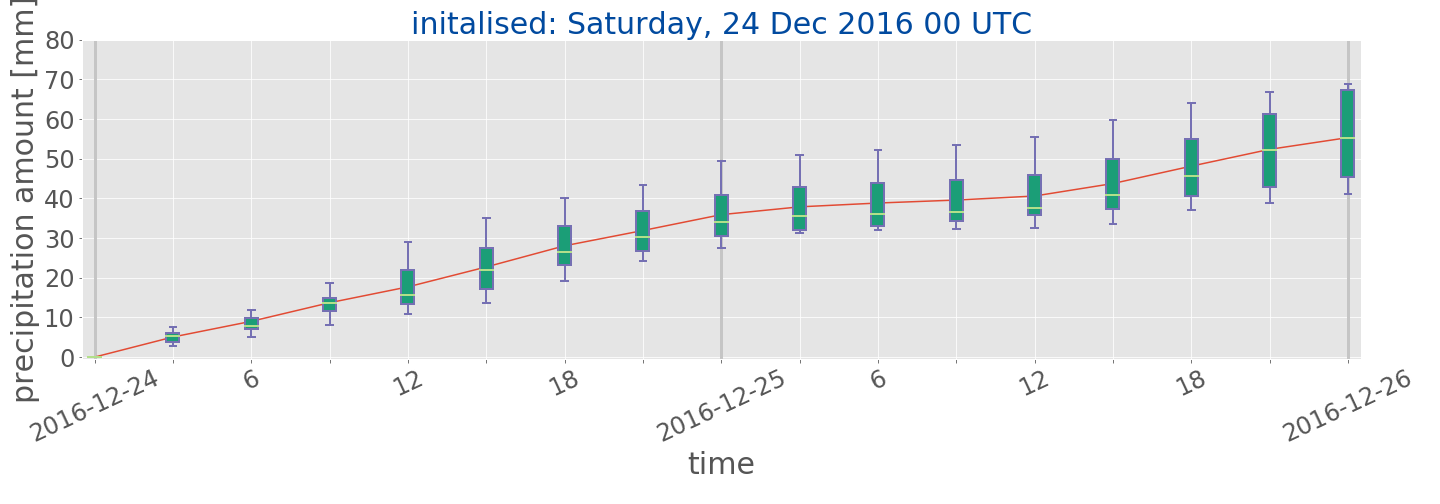
\includegraphics[trim ={0cm 2.2cm 0cm 0cm},clip,width=\textwidth]{./fig_boxplot_sfc/20161224_0}
		\caption{}\label{fig:boxplot:24}
	\end{subfigure}
	%
	\begin{subfigure}[b]{\textwidth}
		\centering
		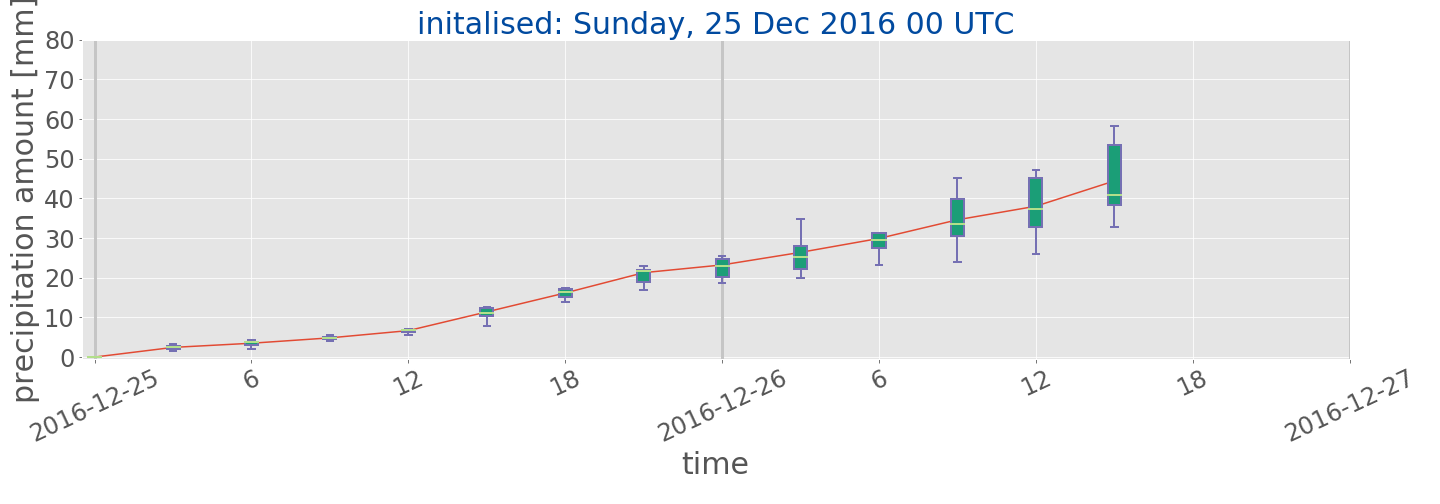
\includegraphics[trim ={0cm 2.2cm 0cm 0cm},clip,width=\textwidth]{./fig_boxplot_sfc/20161225_0}
		\caption{}\label{fig:boxplot:25}
	\end{subfigure}
	%
	\begin{subfigure}[b]{\textwidth}
		\centering
		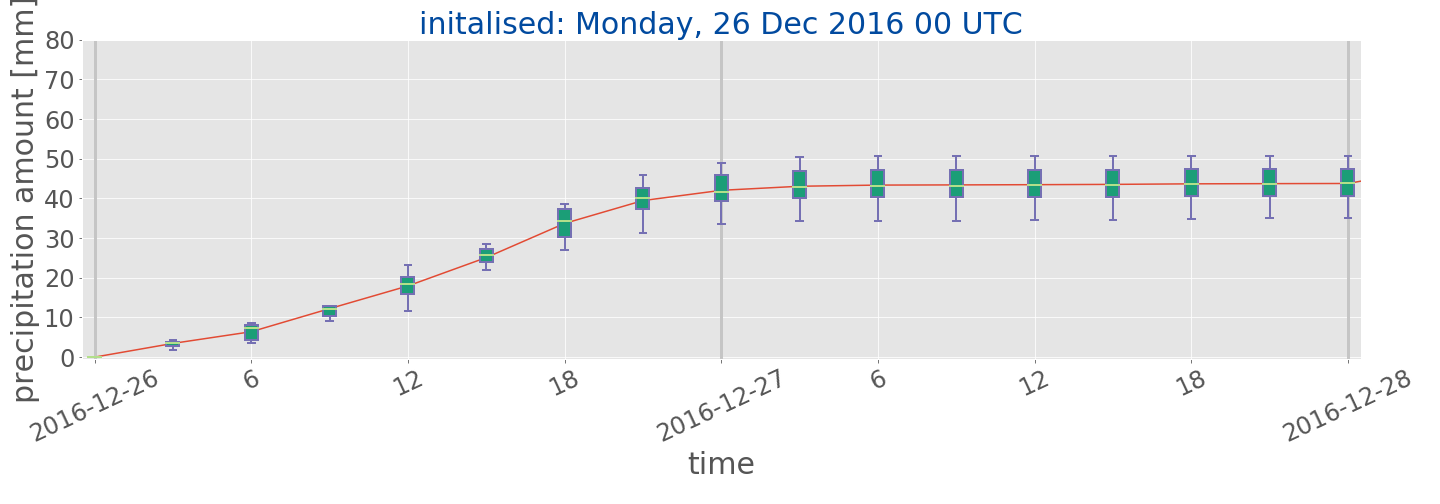
\includegraphics[trim ={0cm 1.cm 0cm 0cm},clip,width=\textwidth]{./fig_boxplot_sfc/20161226_0}
		\caption{}\label{fig:boxplot:26}
	\end{subfigure}
	\caption{Box-whisker-plot of the ten ensemble members of MEPS. Red line indicating the ensemble mean, lower and upper whisker the 25th and 75th percentile, respectively. Light green shows the median of all members and the box represents the middle \SI{50}{\percent} of scores of the precipitation.}\label{fig:boxplot}
\end{figure}
%%%%%%%%%%%%%%%%%%%%%%%%%%%%%%%%%%%%%%%%%%%%%%%%%%%%%%%%%%%%%%%%%%%%%%%%%%
\\
The box-whisker-plot in \Cref{fig:boxplot} shows the distribution of the ten ensemble members for the respective days. All three days with overestimation seem to be different in their variability. As expected increases the forecast uncertainty with longer forecast time for precipitation amount.  
\\
\Cref{fig:boxplot:25} shows for \SI{25}{\dec} the least variability between the ten ensemble members of up to almost \SI{24}{\hour}. The \SI{25}{\dec} is also the forecast with the smallest positive bias of these three days. As \Cref{fig:scat:precip2426} suggests is the overestimation not as high as for \num{24} and \SI{25}{\dec}. On \num{24} and \SI{25}{\dec} is the mean error for the surface accumulation largest with values up to \SI{19}{\mm}. 
\\
Larger variability is already present after \SI{3}{\hour} prediction time in \Cref{fig:boxplot:24} on \SI{24}{\dec}. The spread between the ensemble members (shown by the minimum and maximum whiskers) seems to be wide indicating a larger uncertainty about the amount of surface accumulation. The ensemble mean (red line) is always higher than the median and already after \SI{12}{\hour} forecast time is the median closer to the lower 25th percentile. Also, all upper whiskers in \Cref{fig:boxplot:24} are taller than the lower ones, which would follow that the ensemble members vary amongst the most positive quartile and that it is very similar for the least positive quartile group. Since the deterministic forecast, black line in \Cref{fig:sfc_acc24}, is in the upper percentile compared to its perturbed members it follows that for this forecast the deterministic forecast was not the best guess for the surface accumulation and by using the 'wrong' initial state it can have led to larger miscalculations. 
\\
I believe that the uncertainty appearing already after \SI{3}{\hour} could be associated with a too long spin-up time of MEPS. MEPS usually has a spin-up time of about three hours, on \SI{24}{\dec} this might have been longer as a result of poorer initial conditions \textcolor{red}{Need a reference here, not stated in \citet{muller_arome-metcoop:_2017}}. The regional model MEPS receives initial and boundary conditions from ECMWF before it can produce forecasts \citep{muller_arome-metcoop:_2017}. Since initial conditions such as observations have uncertainties as well as the model has mistrust, and  the own climatology needs to be approached, a model has to stabilize before the simulations can be trusted. The spin-up time varies depending on the quality of the initial and boundary conditions. Apparently, it seems, that the initial and boundary conditions for MEPS were not perfect for initialisations on \SI{24}{\dec} at \SI{0}{\UTC}. The deterministic and perturbed members seem not to have stabilised yet and show larger variability in \Cref{fig:boxplot24} from early on.
\\
The uncertainty might have also been related to the fact, that the large-scale situation got more complex. The precipitation amount associated with the transition of an occluded front on \SI{23}{\dec} was higher than on the previous days (\Cref{fig:res:sfc_precip23} and \Cref{fig:TPU}). On previous days was the hourly precipitation around \SI{0}{\UTC} less intense than on \SI{23}{\dec}. This led to a higher accumulation amount over shorter time and could have followed a larger variability in the forecast model. Another possibility is perhaps that MEPS might have accounted for additional precipitation around \SI{12}{\UTC} on \SI{24}{\dec} and this showed a stronger increase in accretion in \Cref{fig:sfc_acc24} at \SI{13}{\UTC}. I believe it could be associated to a local resolution effect of MEPS. \Cref{fig:meps:site} shows the MEPS resolution and its \SI{2.5}{\km} grid cells around the Haukeliseter site. The complex terrain represented in the model could have followed a local misplacement of a precipitation cell by a few kilometres and followed an estimation of more accumulation at the site after noon.
\\
\\
\Cref{fig:boxplot:25} and \subref{fig:boxplot:26} show a smaller ensemble member variability on \SIlist{25;26}{\dec} than on \SI{24}{\dec}. The box-whiskers are narrower for the first \SI{30}{\hour} in \Cref{fig:boxplot:25}, but slightly larger after \SI{6}{\hour} forecast time for initialisations on \SI{26}{\dec}. \Cref{sec:res:large_scale_sfc} presented a good agreement between observations and forecast of large scale features in terms of pressure, temperature and wind direction. While the occlusion on \SI{26}{\dec} was more intuitive (\Cref{fig:res:sfc_pres26,fig:res:sfc_temp26,fig:res:sfc_wd26,fig:res:sfc_ws26}) than the warm front development on \SI{25}{\dec} (\Cref{fig:res:sfc_pres25}, \subref{fig:res:sfc_temp25}, \subref{fig:res:sfc_wd25}, \subref{fig:res:sfc_ws25}) shows the mean error for each variable to be best for \SI{25}{\dec} (\Cref{fig:MAE:pres},\subref{fig:MAE:temp},\subref{fig:MAE:wd}, \subref{fig:MAE:ws}, and \subref{fig:MAE:precip}).
\\
On \SI{25}{\dec} the overestimation started to occur around \SI{13}{\UTC} in \Cref{fig:sfc_acc25}, related to the delayed forecasted temperature increase in \Cref{fig:res:sfc_temp25}.  As \Cref{fig:boxplot25} shows, increases the variability in the forecast after \SI{15}{\hour} prediction time. In general, agree median and mean well for the entire period of a \SI{48}{\hour} forecast. After \SI{39}{\hour} prediction time is the mean much higher than the median and closer to the lower 25th percentile in \Cref{fig:boxplot25}. It seems, that all ten ensemble members agree well on the prediction and nevertheless overestimates MEPS the surface accumulation. I consider that MEPS misinterpreted the amount of precipitation related to the transition of the warm sector.  
\\
During \SI{26}{\dec} the core of the low-pressure system goes through between \SIlist{15;18}{\UTC} at Haukeliseter. The box-whiskers in \Cref{fig:boxplot:26} indicates a larger variability after \SI{6}{\hour} prediction while the precipitation amount forecast is miscalculated at \SI{12}{\UTC} and following the structure of the double fence observation. Variability of all ensemble members show to increase at \SI{6}{\hour} forecast time, but then decreases again in \Cref{fig:boxplot:26}.  
\\
Since the box-whisker-plot in \Cref{fig:boxplot:25} and \subref{fig:boxplot:26} show less variability in the beginning it is assumed that spin-up time issues are less likely. It could be related to an error in the initialisation state, even though it does not show in the variability in the beginning. An error associated with the spin-up time of MEPS is not totally excluded for these days. In \Cref{fig:sfc_acc25} and \subref{fig:sfc_acc26} agrees the ensemble mean well with the deterministic forecast, which is an indication of a symmetrical spread around the deterministic run. 
\\ 
The overestimation during \num{24} and \SI{26}{\dec} might be related to the high forecasted wind speeds, as well as to the complex development of the low-pressure system north-west of Norway on \SI{24}{\dec}.
\\
%%% table surface accumulation %%%%%%%%%%%%%%%%%%%%%%%%%%%%%%%%%%%%%
\begin{table}[h]
	\begin{center}
		\caption{\textcolor{red}{make new as previous tables} Surface snowfall accumulation measured by the double fence gauge. Presenting \SI{12}{\hour} accumulation before noon and after noon, as well as the total \SI{24}{\hour} surface accretion. }\label{tab:sfc_acc}
		\begin{tabular}{c|c|c|c}
			\hline \hline
			\textbf{Day} & \multicolumn{3}{c}{\textbf{Accumulation}} \\ 
			& \multicolumn{3}{c}{[\SI{}{\mm}]} \\ \hline
			& \SI{12}{\hour} (\footnotesize{\num{0} to \SI{12}{\UTC}}) & \SI{12}{\hour} (\footnotesize{\num{12} to \SI{23}{\UTC}}) & \SI{24}{\hour} \\ \hline \hline
			\SI{21}{\dec} & \num{0.7} &  \num{16.4} & \num{17.1} \\ \hline
			\SI{22}{\dec} & \num{13.6} &  \num{12.0} & \num{25.6} \\ \hline
			\SI{23}{\dec} & \num{6.3} &  \num{17.0} & \num{23.3} \\ \hline
			\SI{24}{\dec} & \num{14.7} &  \num{10.1} & \num{24.8} \\ \hline
			\SI{25}{\dec} & \num{4.3} &  \num{11.1} & \num{15.4} \\ \hline
			\SI{26}{\dec} & \num{8.8} &  \num{16.3} & \num{25.1} \\ 
			\hline \hline
		\end{tabular}
	\end{center}
\end{table}
%%%%%%%%%%%%%%%%%%%%%%%%%%%%%%%%%%%%%%%%%%%%%%%%%%%%%%%%%%%%%%%%%%%%%%%%%%
\\
According to \citet{muller_arome-metcoop:_2017} are strong precipitation events better predicted with AROME-MetCoOp than with ECMWF (European Centre for Medium-Range Weather Forecasts). In \Cref{sec:dim:dec_obs} it was described, that during \num{21} to \SI{27}{\dec} \SI{56.9}{\percent} of the total December 2016 accumulation were observed. \citet{muller_arome-metcoop:_2017} states also, that an overestimation appears, where the precipitation event (\SI{12}{\hour} accumulation) is less than \SI{10}{\mm} this seems not to be true for all days but could be possible for 
\num{25} and \SI{26}{\dec}
(observed accumulation in \Cref{tab:sfc_acc}). In December 2014 was the \SI{12}{\hour} precipitation mean absolute error in AROME-MetCoOp with \SI{1.5}{\mm}. For the Christmas storm is the mean absolute error not larger than \SI{5}{\mm} for the first \SI{12}{\hour} accumulation on \num{24} and \SI{26}{\dec}
(\Cref{fig:MAE:precip12}). Therefore, the assumption follows that on \SI{26}{\dec} the overestimation might be correlated to the <\SI{10}{\mm} problem described by \citet{muller_arome-metcoop:_2017}. The \SI{12}{\hour} accumulation is presented in \Cref{tab:sfc_acc} for Haukeliseter and shows that \SI{12}{\hour} accrection was less than \SI{10}{\mm} for 
\num{25} and \SI{26}{\dec}.
On \SI{25}{\dec} the mean absolute error was \SI{1.1}{\mm} for the first \SI{12}{\hour} accumulation and shows that this could be an influence but does not necessarily mean to be the case, since the overestimation started to occur after \SI{11}{\hour} prediction time. 
\\
\\
% keep as summary in the end
It will be interesting to re-run the ensemble prediction system again with all available observations to see, if this has an influence on the overestimation indicated in \Cref{fig:sfc_acc24,fig:sfc_acc25,fig:sfc_acc26}. ECMWF as boundary condition might not have reached its stabilised state itself when MEPS was initiated and could also have led to a misinterpretation of surface accumulation. A re-run with analysis data from ECMWF could possibly improve the original forecast \textcolor{red}{find reference for this}. 
Another approach could be to perturb the initial state (deterministic forecast) in other way, to see if different perturbations might lead to a better correlation between observation and forecast at the ground than presented in \Cref{fig:scat:precip2124}. Also, the deterministic forecast (best guess) might have been chosen incorrectly and followed a miscalculation of surface accumulation, since the misinterpreted best guess was perturbed.
It is very important to have correct measurements such as the double fence or MRR observations, to produce better initial condition for weather forecast models, so that initialisations can start at a realistic state.
\\
Also, more study cases should be considered to get a better estimate about the performance of MEPS during extreme winter events. The mean absolute error for \SI{12}{\hour} accumulation has shown a great variability, depending on the initialisation time and the intensification of the low-pressure system.  
%%%%%%%%%%%%%%%%%%%%%%%%%%%%%%%%%%%%%%%%%%%%%%%%%%%%%%%%%%%%%%%%%%%%%%%%%%




